\UseRawInputEncoding
\documentclass{report}
\usepackage{url}
\usepackage{mdframed}
\usepackage{graphicx}
\usepackage{xspace}
\usepackage[utf8]{inputenc} % Ensure UTF-8 input encoding
\usepackage[T1]{fontenc}
\usepackage{amsmath}
\usepackage{listings} % For code formatting

% Configuration for code listings
\lstset{
    basicstyle=\ttfamily\small,
    frame=single,
    numbers=left,
    numberstyle=\tiny,
    keywordstyle=\color{blue}\bfseries,
    commentstyle=\color{gray},
    stringstyle=\color{red},
    showstringspaces=false,
    breaklines=true,
    postbreak=\mbox{\textcolor{red}{$\hookrightarrow$}\space},
    tabsize=2
}

\begin{document}

\begin{titlepage}
\centering
\vspace*{\fill}
\huge{\textbf{CS3008: IMAGE AND VIDEO PROCESSING}}\\
\vspace{1 cm}

\begin{mdframed}
\centering
\LARGE{\textbf{LABORATORY REPORTS}}
\end{mdframed}

\vspace{3 cm}

\begin{flushleft}
\large{\textbf{Name: Jayashre\\
Roll No.: 22011103020 \\
College: Shiv Nadar University, Chennai\\}}

\vspace*{\fill}

\end{flushleft}
\end{titlepage}

\chapter{Eye Detection Using OpenCV} % Enable numbering for chapter

\section{Abstract}
This report documents the implementation of an eye detection system using the OpenCV library. The system utilizes Haar cascade classifiers to identify faces and eyes in images and marks them with bounding boxes. The project aims to provide a foundational understanding of image processing techniques and their practical applications.

\section{Introduction}
Eye detection plays a vital role in computer vision applications such as gaze tracking, facial recognition, and user interaction systems. This project implements a detection system using pre-trained Haar cascade classifiers, which efficiently identify facial and ocular features in images.

\section{Methodology}
\subsection{Data Collection}
The input data consists of static images containing human faces. The images were uploaded manually in the Google Colab environment for processing.

\subsection{Tools and Libraries}
\begin{itemize}
    \item \textbf{OpenCV}: For image processing and detection.
    \item \textbf{Google Colab}: For executing Python code and visualizing results.
\end{itemize}

\subsection{Detection Algorithm}
The steps followed in the implementation are:
\begin{enumerate}
    \item Convert the input image to grayscale for easier processing.
    \item Use the Haar cascade classifier to detect faces in the image.
    \item For each detected face, apply the Haar cascade classifier for eyes within the facial region.
    \item Highlight the detected features (faces and eyes) using bounding boxes.
\end{enumerate}

\section{Implementation}
The implementation was carried out in Python using OpenCV. The following code snippet demonstrates the detection process:

\begin{lstlisting}[language=Python, caption=Eye Detection Code, label=code:eye-detection]
import cv2
face_cascade = cv2.CascadeClassifier(cv2.data.haarcascades + 'haarcascade_frontalface_default.xml')
eye_cascade = cv2.CascadeClassifier(cv2.data.haarcascades + 'haarcascade_eye.xml')
image = cv2.imread('input_image.jpg')
gray_image = cv2.cvtColor(image, cv2.COLOR_BGR2GRAY)
faces = face_cascade.detectMultiScale(gray_image, scaleFactor=1.1, minNeighbors=5)

for (x, y, w, h) in faces:
    cv2.rectangle(image, (x, y), (x+w, y+h), (255, 0, 0), 2)
    roi_gray = gray_image[y:y+h, x:x+w]
    roi_color = image[y:y+h, x:x+w]
    eyes = eye_cascade.detectMultiScale(roi_gray)
    for (ex, ey, ew, eh) in eyes:
        cv2.rectangle(roi_color, (ex, ey), (ex+ew, ey+eh), (0, 255, 0), 2)
cv2.imwrite('output_image.jpg', image)
cv2.imshow('Eye Detection', image)
cv2.waitKey(0)
cv2.destroyAllWindows()
\end{lstlisting}

\section{Results and Discussion}
The system was tested with several images under various conditions. The results are summarized below:
\begin{itemize}
    \item Faces were detected accurately in well-lit images.
    \item Eye detection was successful but occasionally struggled with images where faces were partially obscured.
\end{itemize}

\begin{figure}[h!]
    \centering
    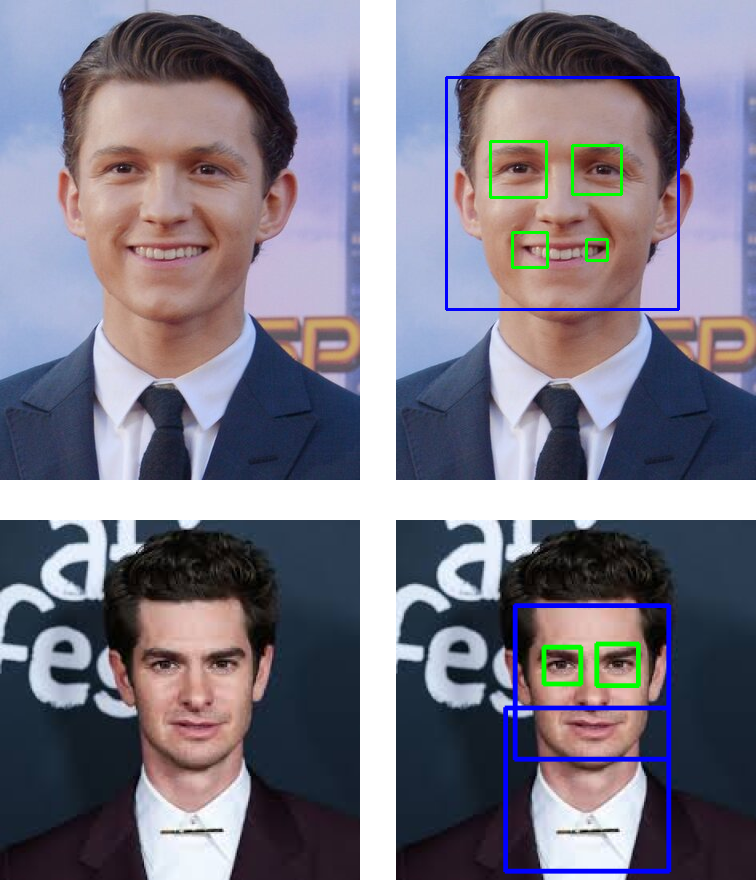
\includegraphics[width=0.4\textwidth]{images/Exp-1-Results.png} % Adjusted image size
    \caption{Detected faces and eyes in the input image.}
    \label{fig:output}
\end{figure}

\section{Conclusion}
The project successfully implemented an eye detection system using Haar cascades in OpenCV. While the system is efficient for basic detection, future improvements can involve the use of deep learning-based models for enhanced accuracy and robustness.

\chapter{Image Processing and Effects} % Enable numbering for chapter

\section{Abstract}
This report documents the implementation of various image processing techniques, including applying filters, resizing, cropping, rotating, and face mask overlays. These tasks showcase the practical applications of computer vision and image manipulation using Python and OpenCV.

\section{Introduction}
Image processing is a cornerstone of computer vision, enabling tasks like object detection, image enhancement, and feature extraction. This project demonstrates the use of OpenCV to apply filters and transformations to images, and overlay masks on detected faces.

\section{Methodology}
\subsection{Data Collection}
The input data consists of static images uploaded manually in the Google Colab environment. 

\subsection{Tools and Libraries}
\begin{itemize}
    \item \textbf{OpenCV}: For image processing and transformations.
    \item \textbf{Google Colab}: For executing Python code and visualizing results.
    \item \textbf{NumPy}: For handling numerical operations.
\end{itemize}

\subsection{Image Processing Techniques}
The project implements the following techniques:
\begin{itemize}
    \item Grayscale, sepia, negative, and blur effects.
    \item Edge detection and cartoonification.
    \item Image resizing, cropping, and rotation.
\end{itemize}

\section{Implementation}
The implementation was carried out in Python using OpenCV. The following code snippet demonstrates the overall process:

\begin{lstlisting}[language=Python, caption=Image Processing Code, label=code:image-processing]
import cv2
import numpy as np
from google.colab.patches import cv2_imshow

image_path = "content/sample.png"
img = cv2.imread(image_path)

def apply_grayscale(image):
    return cv2.cvtColor(image, cv2.COLOR_BGR2GRAY)

def apply_sepia(image):
    kernel = np.array([[0.393, 0.769, 0.189],
                       [0.349, 0.686, 0.168],
                       [0.272, 0.534, 0.131]])
    return cv2.transform(image, kernel)

def apply_negative(image):
    return cv2.bitwise_not(image)

def apply_blur(image, ksize=(5, 5)):
    return cv2.GaussianBlur(image, ksize, 0)

def apply_edge_detection(image):
    return cv2.Canny(image, 100, 200)

def apply_cartoonify(image):
    gray = cv2.cvtColor(image, cv2.COLOR_BGR2GRAY)
    gray = cv2.medianBlur(gray, 5)
    edges = cv2.adaptiveThreshold(gray, 255, cv2.ADAPTIVE_THRESH_MEAN_C, cv2.THRESH_BINARY, 9, 9)
    color = cv2.bilateralFilter(image, 9, 300, 300)
    return cv2.bitwise_and(color, color, mask=edges)

def resize_image(image, width=500):
    aspect_ratio = width / float(image.shape[1])
    height = int(image.shape[0] * aspect_ratio)
    return cv2.resize(image, (width, height))

def crop_image(image):
    height, width = image.shape[:2]
    size = min(height, width)
    center_x, center_y = width // 2, height // 2
    cropped = image[center_y - size // 2:center_y + size // 2, center_x - size // 2:center_x + size // 2]
    return cropped

def rotate_image(image, angle=45):
    height, width = image.shape[:2]
    center = (width // 2, height // 2)
    matrix = cv2.getRotationMatrix2D(center, angle, 1)
    rotated = cv2.warpAffine(image, matrix, (width, height))
    return rotated


grayscale_img = apply_grayscale(img)
sepia_img = apply_sepia(img)
negative_img = apply_negative(img)
blur_img = apply_blur(img)
edges_img = apply_edge_detection(img)
cartoon_img = apply_cartoonify(img)
resized_img = resize_image(img)
cropped_img = crop_image(img)
rotated_img = rotate_image(img)

cv2_imshow(grayscale_img)
cv2_imshow(sepia_img)
cv2_imshow(negative_img)
cv2_imshow(blur_img)
cv2_imshow(edges_img)
cv2_imshow(cartoon_img)
cv2_imshow(resized_img)
cv2_imshow(cropped_img)
cv2_imshow(rotated_img)
\end{lstlisting}

\section{Results and Discussion}
The following observations were made during testing:
\begin{itemize}
    \item Filters like grayscale, sepia, and negative worked as expected.
    \item Cartoonification produced visually appealing results by emphasizing edges.
\end{itemize}

\begin{figure}[h!]
    \centering
    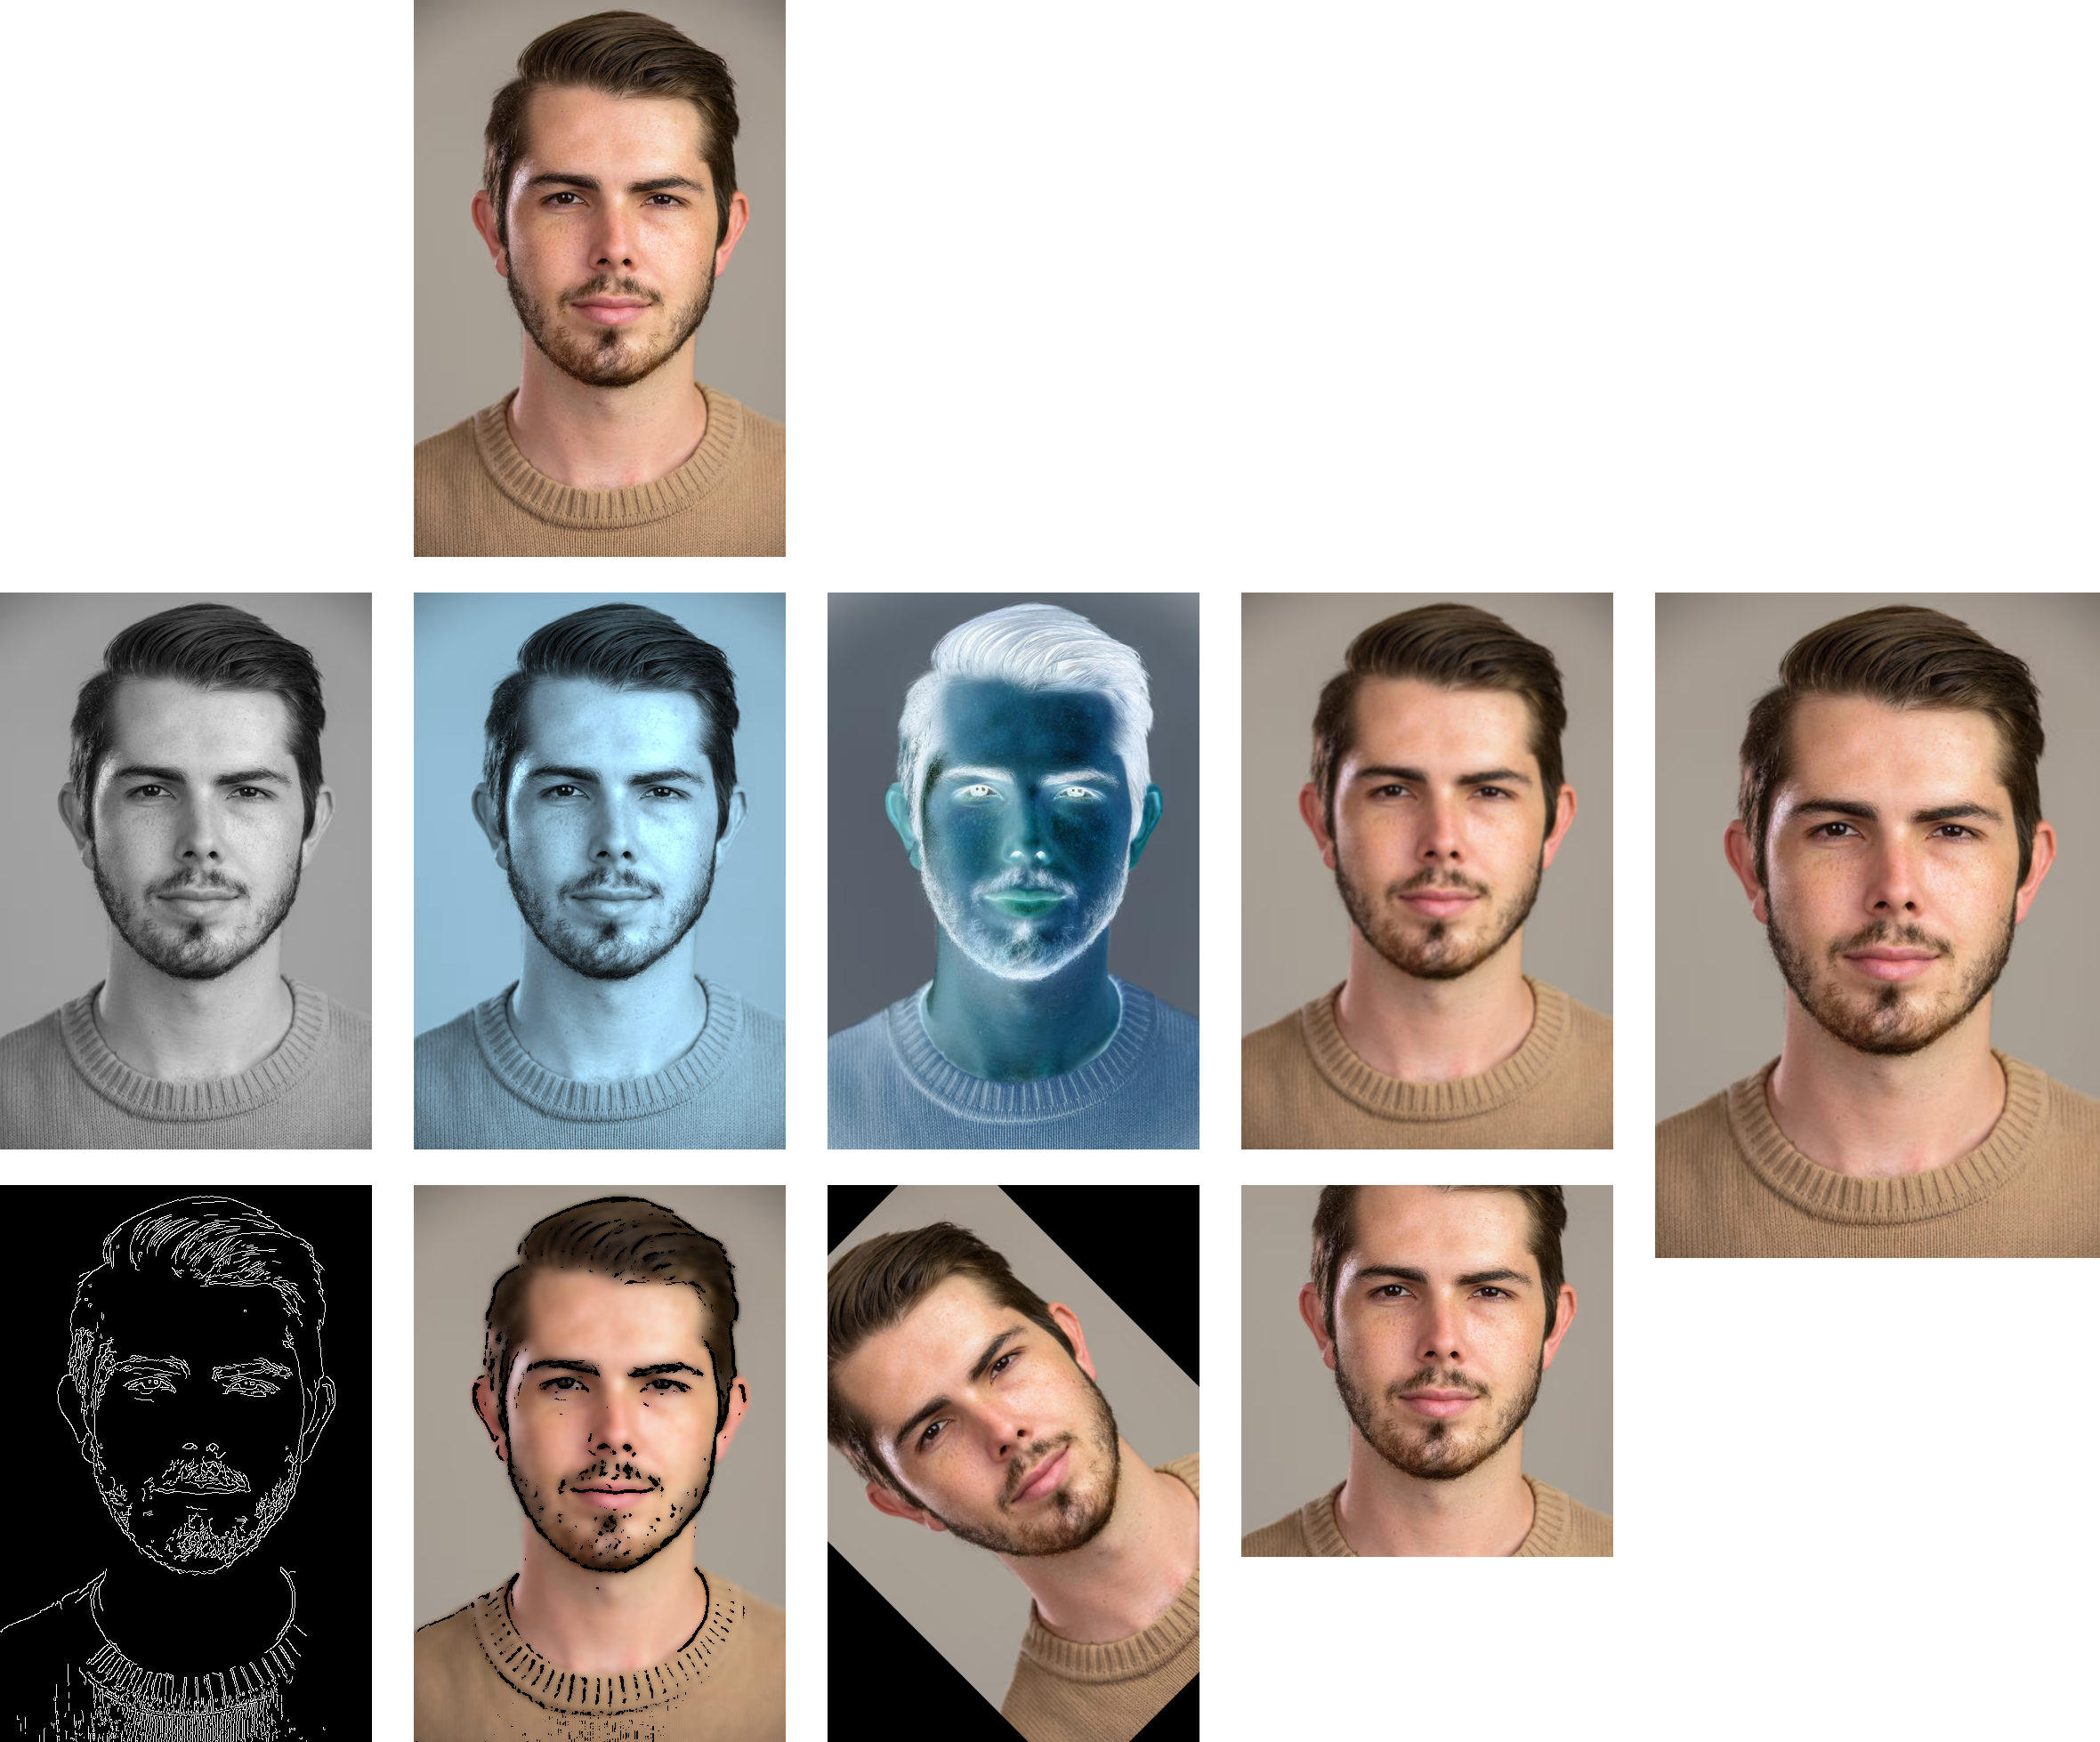
\includegraphics[width=0.4\textwidth]{images/Exp-2-Results.png} % Adjusted image size
    \caption{Examples of applied filters and transformations.}
    \label{fig:output}
\end{figure}

\section{Conclusion}
This project successfully demonstrated various image processing techniques using OpenCV. Future work could explore integrating deep learning models for more advanced image transformations and processing.

\chapter{Image Resolution and Interpolation Studies} % Enable numbering for chapter

\section{Abstract}
This report explores the fundamental concepts of image resolution and interpolation in image processing. The experiments involve converting RGB images to grayscale using a formula, analyzing intensity and spatial resolution changes, and studying image interpolation techniques. The study aims to provide insights into how image transformations affect visual quality and data representation.

\section{Introduction}
Image resolution and interpolation are critical aspects of image processing. Resolution defines the level of detail in an image, while interpolation determines how images are scaled to different dimensions. This project investigates these aspects through practical implementations and analyses their impact on image quality.

\section{Methodology}
\subsection{Tools and Libraries}
\begin{itemize}
    \item \textbf{OpenCV}: For image processing operations.
    \item \textbf{NumPy}: For numerical computations.
    \item \textbf{Google Colab}: For implementation and visualization.
\end{itemize}

\subsection{Experiments Conducted}
\begin{enumerate}
    \item \textbf{Convert RGB to Grayscale:} An RGB image is converted to grayscale using the formula:
    \[ Y = 0.299 \cdot R + 0.587 \cdot G + 0.114 \cdot B \]

    \item \textbf{Intensity Resolution:} An 8-bit grayscale image is converted into 7, 6, 5, 4, 3, and 2-bit images by reducing the bit depth and analyzing the resulting quality loss.

    \item \textbf{Spatial Resolution:} A 512x512 image is resized to 256x256, 128x128, 64x64, and 32x32 dimensions to observe the effect of reduced spatial resolution.

    \item \textbf{Image Interpolation:} A 128x128 image is resized to 256x256 and 512x512 dimensions using bilinear and bicubic interpolation techniques.
\end{enumerate}

\section{Implementation}
The implementation was carried out using Python and OpenCV. The following snippets showcase the key operations:

\begin{lstlisting}[language=Python, caption=Convert RGB to Grayscale, label=code:grayscale]
import cv2
import numpy as np
import matplotlib.pyplot as plt

image = cv2.imread('/content/image.jpg')

image_rgb = cv2.cvtColor(image, cv2.COLOR_BGR2RGB)

R = image_rgb[:, :, 0]
G = image_rgb[:, :, 1]
B = image_rgb[:, :, 2]

gray_image = 0.299 * R + 0.587 * G + 0.114 * B
gray_image = gray_image.astype(np.uint8)

plt.imshow(gray_image, cmap='gray')
plt.title("Grayscale Image (Formula)")
plt.axis('off')
plt.show()
\end{lstlisting}

\begin{lstlisting}[language=Python, caption=Bit Depth Reduction, label=code:intensity-resolution]
import numpy as np
import cv2
import matplotlib.pyplot as plt

image = cv2.imread('/content/image.jpg', cv2.IMREAD_GRAYSCALE)

def reduce_intensity_resolution(image, bits):
    max_intensity = 2**bits - 1
    return np.uint8((image / 256) * max_intensity)

bit_depths = [7, 6, 5, 4, 3, 2]
for bits in bit_depths:
    reduced_image = reduce_intensity_resolution(image, bits)
    plt.imshow(reduced_image, cmap='gray')
    plt.title(f"{bits}-bit Image")
    plt.axis('off')
    plt.show()
\end{lstlisting}

\begin{lstlisting}[language=Python, caption=Spatial Resolution Adjustment, label=code:spatial-resolution]
import cv2
import matplotlib.pyplot as plt

image = cv2.imread('/content/penguin.jpg', cv2.IMREAD_GRAYSCALE)

def resize_image(image, size):
    return cv2.resize(image, (size, size), interpolation=cv2.INTER_LINEAR)

sizes = [256, 128, 64, 32]
for size in sizes:
    resized_image = resize_image(image, size)
    plt.imshow(resized_image, cmap='gray')
    plt.title(f"{size}x{size} Image")
    plt.axis('off')
    plt.show()
    cv2.imwrite(f'{size}x{size}_image.jpg', resized_image)
\end{lstlisting}

\begin{lstlisting}[language=Python, caption=Image Interpolation, label=code:interpolation]
import cv2
import matplotlib.pyplot as plt

image = cv2.imread('/content/sunset.jpg', cv2.IMREAD_GRAYSCALE)

def upscale_image(image, new_size, interpolation_method):
    return cv2.resize(image, (new_size, new_size), interpolation=interpolation_method)
interpolation_methods = {
    'Nearest Neighbor': cv2.INTER_NEAREST,
    'Bilinear': cv2.INTER_LINEAR,
    'Bicubic': cv2.INTER_CUBIC
}

sizes = [256, 512]
for size in sizes:
    for method_name, method in interpolation_methods.items():
        upscaled_image = upscale_image(image, size, method)
        plt.imshow(upscaled_image, cmap='gray')
        plt.title(f"{size}x{size} Image with {method_name} Interpolation")
        plt.axis('off')
        plt.show()
        cv2.imwrite(f'{size}x{size}_{method_name}_interpolation.jpg', upscaled_image)
\end{lstlisting}

\section{Results and Discussion}
\subsection{RGB to Grayscale}
The grayscale conversion effectively reduced the color data of the image while preserving its luminance, demonstrating the precision of the formula.

\subsection{Intensity Resolution}
The reduction in bit depth showed a gradual loss in image quality. Higher bit depths retained more details, while lower depths introduced noticeable quantization artifacts.

\subsection{Spatial Resolution}
Decreasing the spatial resolution led to a loss of detail and sharpness. However, the images remained recognizable at lower resolutions, demonstrating the trade-off between quality and storage requirements.

\subsection{Image Interpolation}
Bilinear and bicubic interpolation effectively upscaled the images. Bicubic interpolation provided smoother results but required higher computational resources compared to bilinear interpolation.

\begin{figure}[h!]
    \centering
    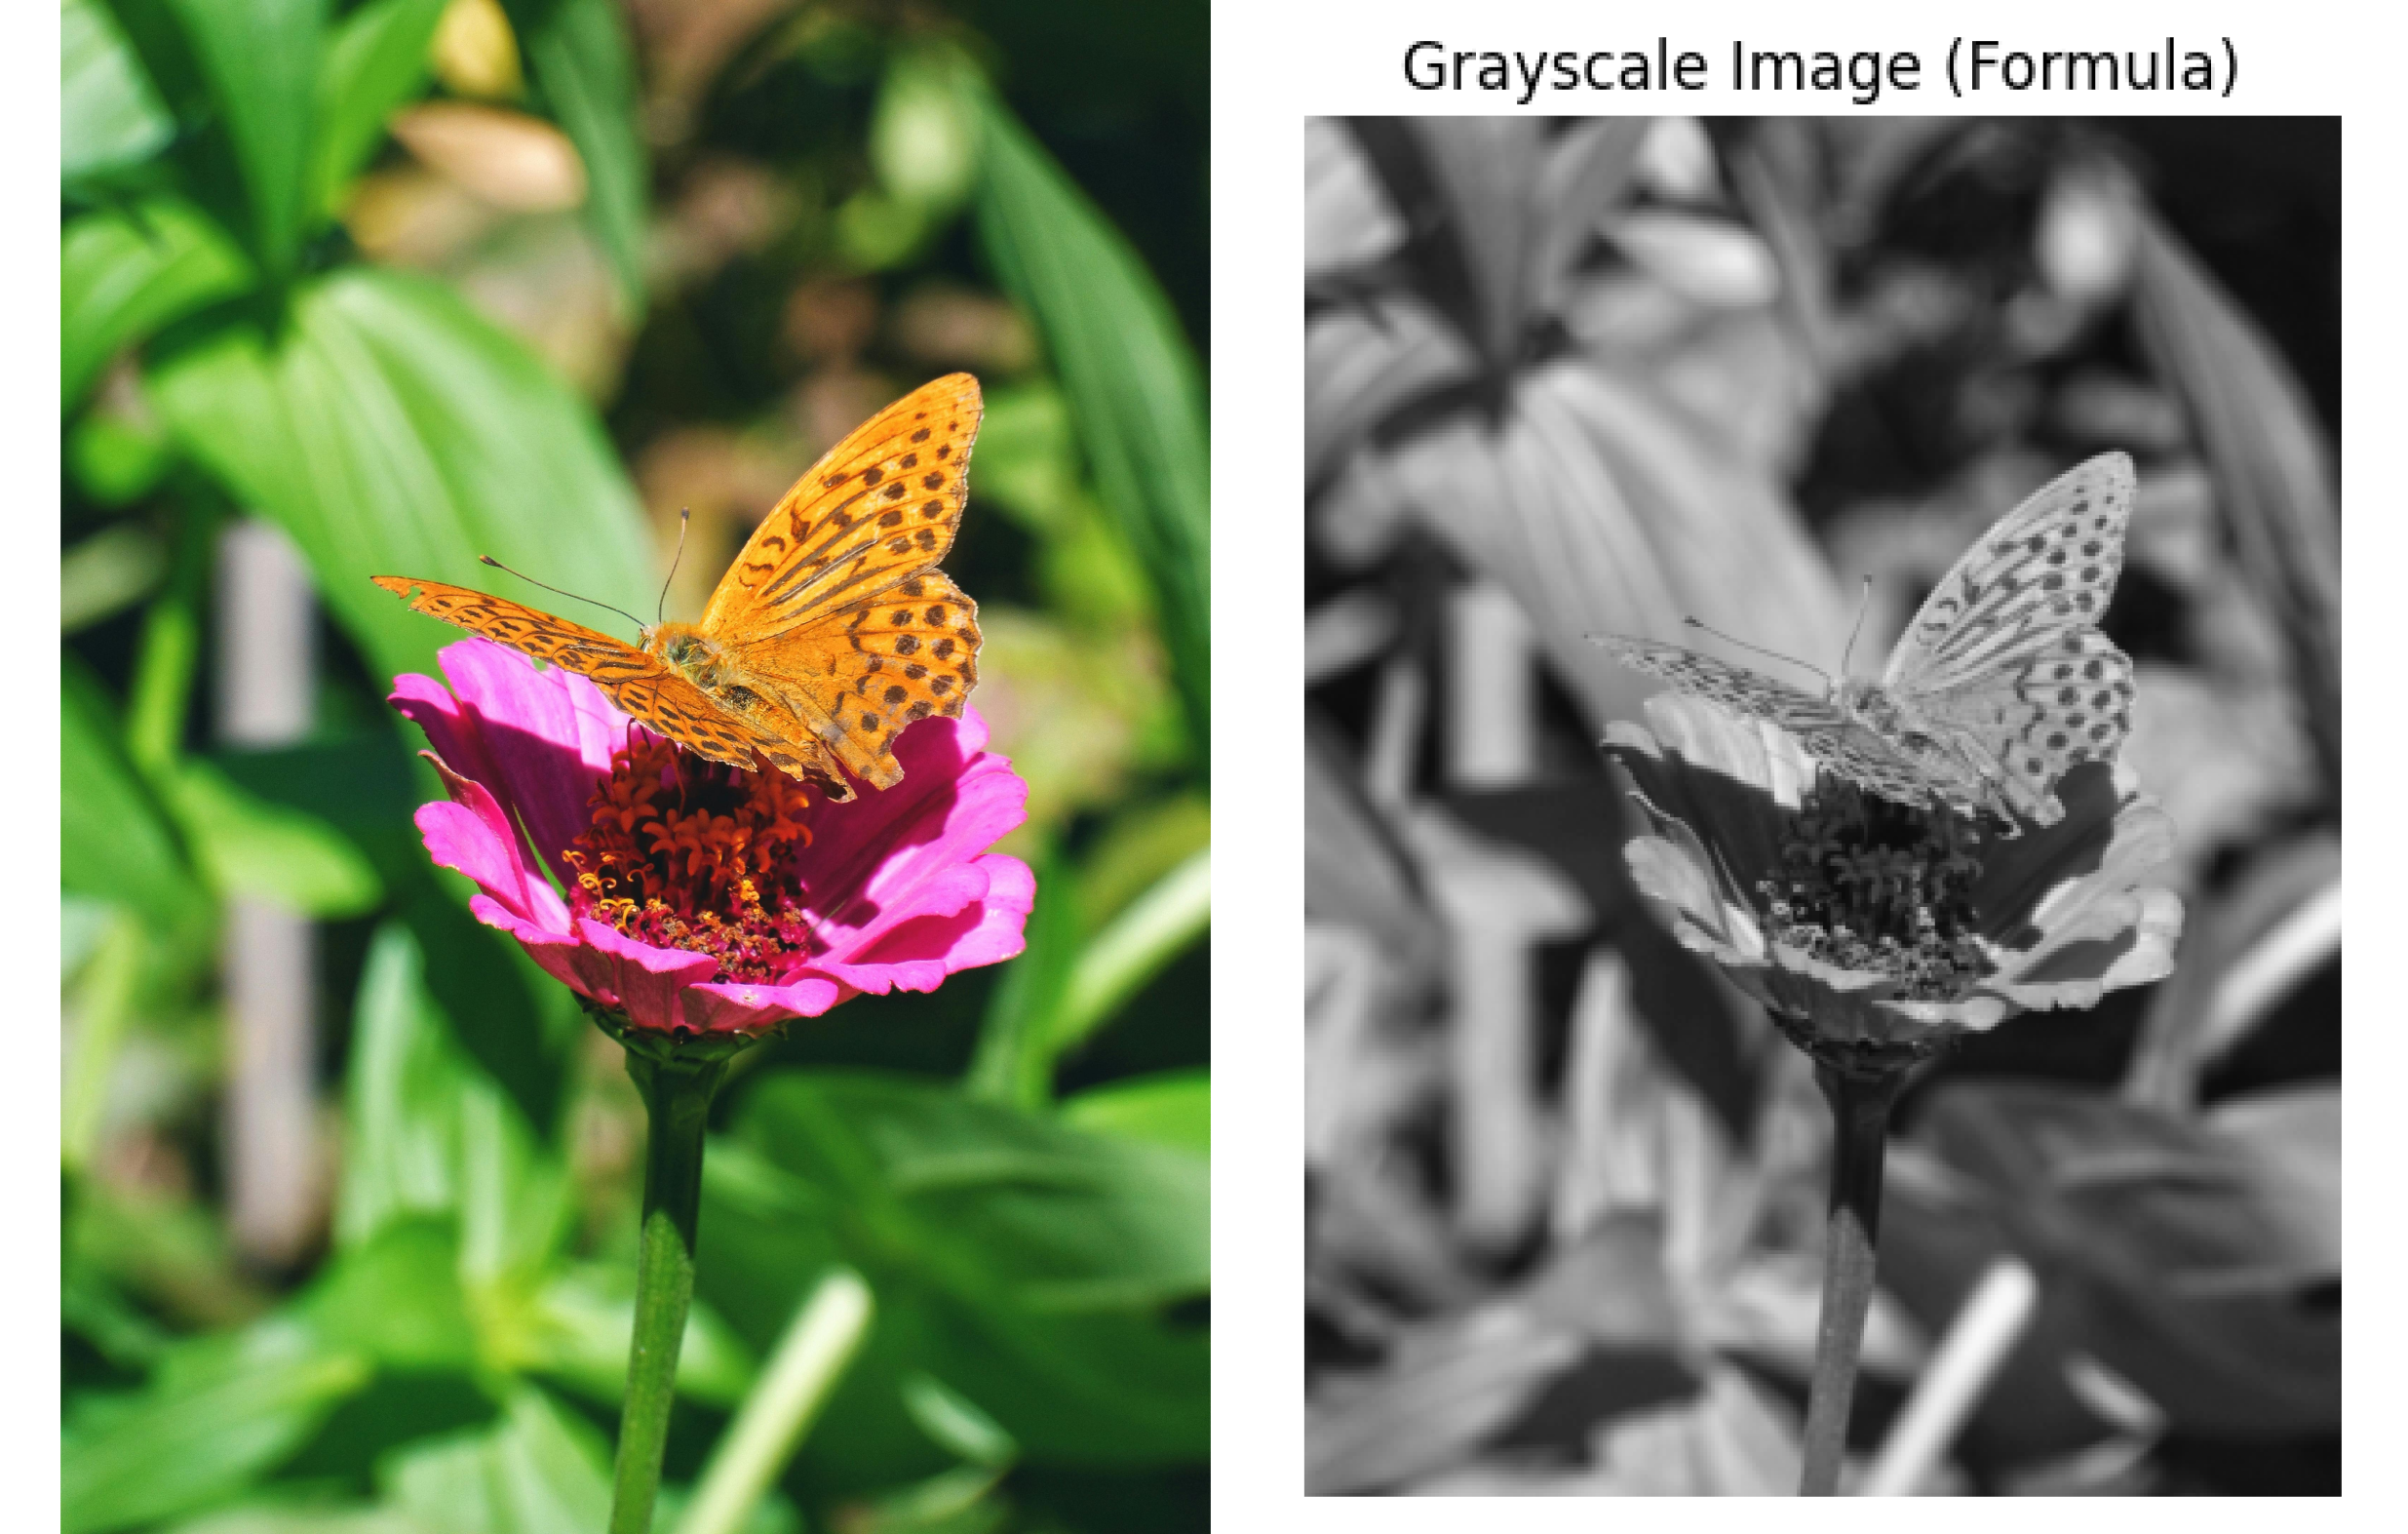
\includegraphics[width=0.4\textwidth]{images/Exp-3-Results-1.png} % Placeholder for results image
    \caption{Conversion RGB to Grayscale}
    \label{fig:exp-3-results}
\end{figure}

\begin{figure}[h!]
    \centering
    \includegraphics[width=0.4\textwidth]{images/Exp-3-Results-2.png} % Placeholder for results image
    \caption{Intensity Resolution.}
    \label{fig:exp-3-results}
\end{figure}

\begin{figure}[h!]
    \centering
    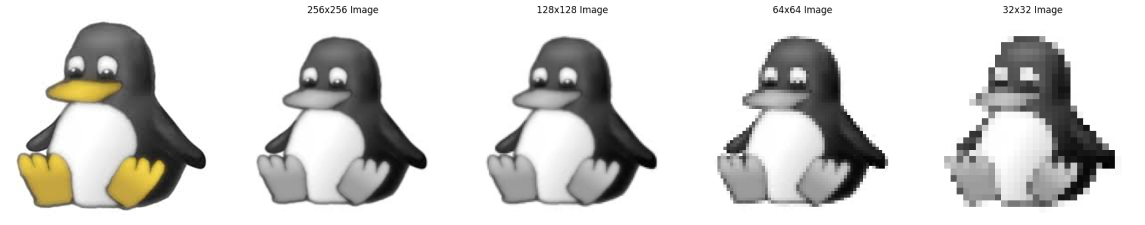
\includegraphics[width=0.4\textwidth]{images/Exp-3-Results-3.png} % Placeholder for results image
    \caption{Spatial Resolution.}
    \label{fig:exp-3-results}
\end{figure}

\begin{figure}[h!]
    \centering
    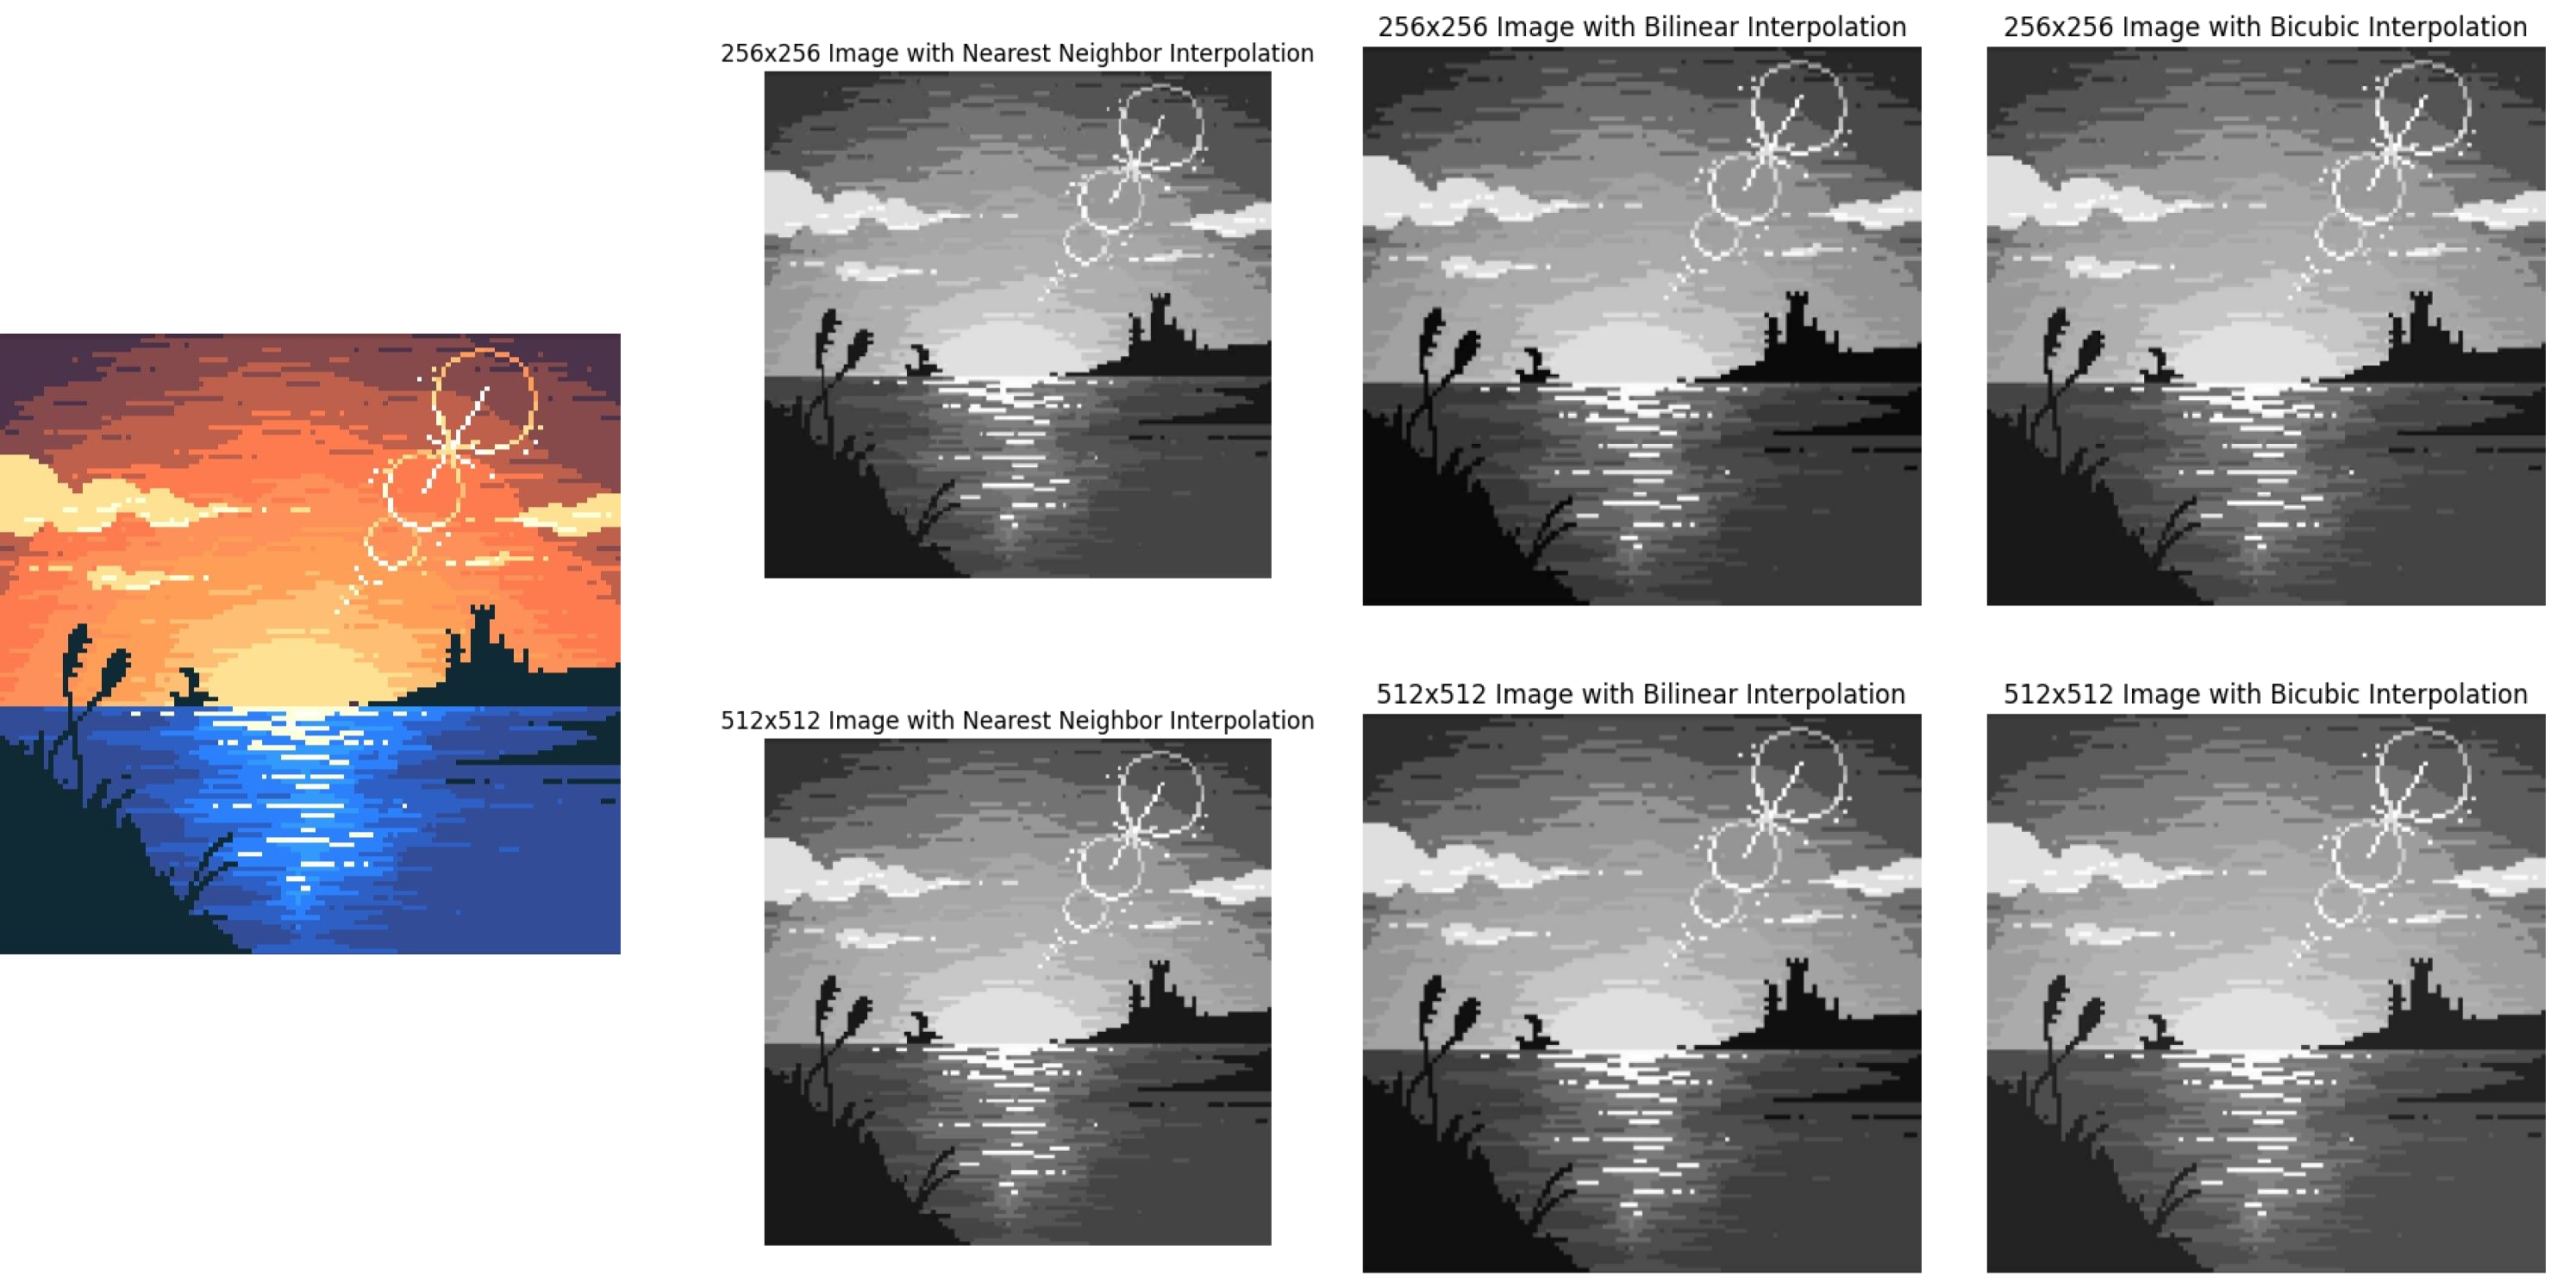
\includegraphics[width=0.4\textwidth]{images/Exp-3-Results-4.png} % Placeholder for results image
    \caption{Image Interpolation.}
    \label{fig:exp-3-results}
\end{figure}

\section{Conclusion}
The experiments provided insights into how resolution and interpolation affect image quality. Future work can involve exploring advanced interpolation techniques, such as deep learning-based methods, for higher accuracy and efficiency.

\chapter{Filtering and Blurring Techniques}

\section{Abstract}
This report details the experiments conducted in Week 4 of the laboratory exercises, focusing on filtering and blurring techniques. Various filters, including box and Gaussian filters, were applied, and concepts like correlation, convolution, and separable filters were studied.

\section{Introduction}
Image filtering and blurring techniques are fundamental operations in image processing. These techniques enhance image quality, simulate natural effects, or prepare images for further analysis. The aim of this experiment was to explore these techniques using different filters and kernel configurations.

\section{Methodology}

\subsection{Box Filter}
A box filter was applied with different kernel sizes (e.g., 3x3, 5x5, 7x7, 9x9, 11x11, 13x13, 15x15). The filtering process involved averaging the pixel values within the kernel to produce a smoothed image.

\subsection{Defocus Blur Simulation}
Defocus blur was simulated by applying a circular averaging filter to mimic the effect of an out-of-focus lens.

\subsection{Motion Blur}
A motion blur kernel was designed to simulate the effect of camera motion. The kernel was applied to the image using convolution.

\subsection{Correlation vs Convolution}
The experiment compared the results of correlation and convolution operations on the same image, highlighting the differences in their mathematical operations and outcomes.

\subsection{Separable Filters}
Separable filters were studied and implemented. A 2D filter was decomposed into two 1D filters for computational efficiency.

\subsection{Gaussian Distribution}
Gaussian filters with varying sigma values (e.g., 0.5, 1, 2) were applied. The Gaussian kernel had a mean of 0 and was constructed using the formula:
\begin{equation}
G(x, y) = \frac{1}{{2\pi\sigma^2}} e^{-\frac{x^2 + y^2}{2\sigma^2}}
\end{equation}

\section{Implementation}
The implementation details for each task are summarized below:
\subsection{Box Filter}
\begin{lstlisting}[language=Python, caption=Box Filter Implementation]
import cv2
import numpy as np
import matplotlib.pyplot as plt
image = cv2.imread('sample.jpeg', cv2.IMREAD_GRAYSCALE)
kernel_sizes = [3, 5, 7, 9, 11, 13, 15]
filtered_images = []

for size in kernel_sizes:
    kernel = np.ones((size, size), np.float32) / (size * size)
    filtered = cv2.filter2D(image, -1, kernel)
    filtered_images.append(filtered)

plt.figure(figsize=(12, 6))
for i, filtered in enumerate(filtered_images):
    plt.subplot(1, len(filtered_images), i + 1)
    plt.title(f"Kernel: {kernel_sizes[i]}x{kernel_sizes[i]}")
    plt.imshow(filtered, cmap='gray')
    plt.axis('off')
plt.show()
\end{lstlisting}

\subsection{Defocus Blur}
\begin{lstlisting}[language=Python, caption=Defocus Blur Simulation]
image = cv2.imread('sample.jpeg', cv2.IMREAD_GRAYSCALE)
def circular_kernel(radius):
    y, x = np.ogrid[-radius:radius+1, -radius:radius+1]
    mask = x**2 + y**2 <= radius**2
    kernel = np.zeros_like(mask, dtype=np.float32)
    kernel[mask] = 1
    kernel /= kernel.sum()
    return kernel
radius = [20, 25, 30, 35, 40, 45]
for rad in radius:
  kernel = circular_kernel(rad)
  blurred_image = cv2.filter2D(image, -1, kernel)
  plt.figure(figsize=(6, 6))
  plt.title(f"Defocus Blur with Radius {rad}")
  plt.imshow(blurred_image, cmap='gray')
  plt.axis('off')
  plt.show()
\end{lstlisting}

\subsection{Motion Blur}
\begin{lstlisting}[language=Python, caption=Motion Blur Implementation]
image = cv2.imread('sample.jpeg', cv2.IMREAD_GRAYSCALE)
def motion_blur_kernel(size, angle):
    kernel = np.zeros((size, size), dtype=np.float32)
    mid = size // 2
    if angle == 0:
        kernel[mid, :] = 1
    elif angle == 90:
        kernel[:, mid] = 1
    elif angle == 45:
        np.fill_diagonal(kernel, 1)
    else:
        raise ValueError("Only angles 0, 90, and 45 are supported")
    kernel /= kernel.sum()
    return kernel
kernel_size = [35, 45, 55, 65]
angle = 0
for ker in kernel_size:
  kernel = motion_blur_kernel(ker, angle)
  motion_blurred_image = cv2.filter2D(image, -1, kernel)
  plt.figure(figsize=(6, 6))
  plt.title(f"Motion Blur wi th Kernel Size {ker}, Angle {angle}\textdegree")
  plt.imshow(motion_blurred_image, cmap='gray')
  plt.axis('off')
  plt.show()
\end{lstlisting}

\subsection{Correlation vs Convolution}
\begin{lstlisting}[language=Python, caption=Correlation and Convolution Study]
from scipy import ndimage
image = cv2.imread('sample.jpeg', 0)
kernel = np.array([[1,1,1],[1,1,0],[1,0,0]])
convolved_image = ndimage.convolve(image, kernel, mode='constant', cval=1.0)
correlated_image = cv2.filter2D(image, -1, kernel)
plt.figure(figsize=(12, 6))
plt.subplot(1, 2, 1)
plt.title("Convolution")
plt.imshow(convolved_image, cmap='gray')
plt.axis('off')
plt.subplot(1, 2, 2)
plt.title("Correlation")
plt.imshow(correlated_image, cmap='gray')
plt.axis('off')
plt.show()

\end{lstlisting}

\subsection{Separable Filters}
\begin{lstlisting}[language=Python, caption=Separable Filter Implementation]
import cv2
import numpy as np
image = cv2.imread('input_image.jpg', 0)
kernel = np.outer([1, 2, 1], [1, 2, 1])
kernel = kernel / kernel.sum()
separable_result = cv2.sepFilter2D(image, -1, kernel, kernel)
cv2.imwrite('separable_filter_output.jpg', separable_result)
\end{lstlisting}

\subsection{Gaussian Distribution}
\begin{lstlisting}[language=Python, caption=Gaussion Distribution]
import numpy as np
import matplotlib.pyplot as plt
mu = 0  # Mean
sigma_values = [0.5, 1.0, 1.5, 2.0, 2.5,]
x = np.linspace(-5, 5, 1000)
plt.figure(figsize=(10, 6))
for sigma in sigma_values:
    y = 1/(sigma * np.sqrt(2 * np.pi)) * np.exp(-(x - mu)**2 / (2 * sigma**2))
    plt.plot(x, y, label=f'Sigma = {sigma}')
plt.title('Gaussian Distribution with Mean 0 and Different Sigma Values')
plt.xlabel('X')
plt.ylabel('Probability density')
plt.legend()
plt.grid(True)
plt.show()
\end{lstlisting}

\section{Results and Discussion}
The results of the filtering and blurring techniques were as follows:
\begin{itemize}
    \item Box filtering effectively smoothed the image, with larger kernel sizes producing stronger effects.
    \begin{figure}[h!]
    \centering
    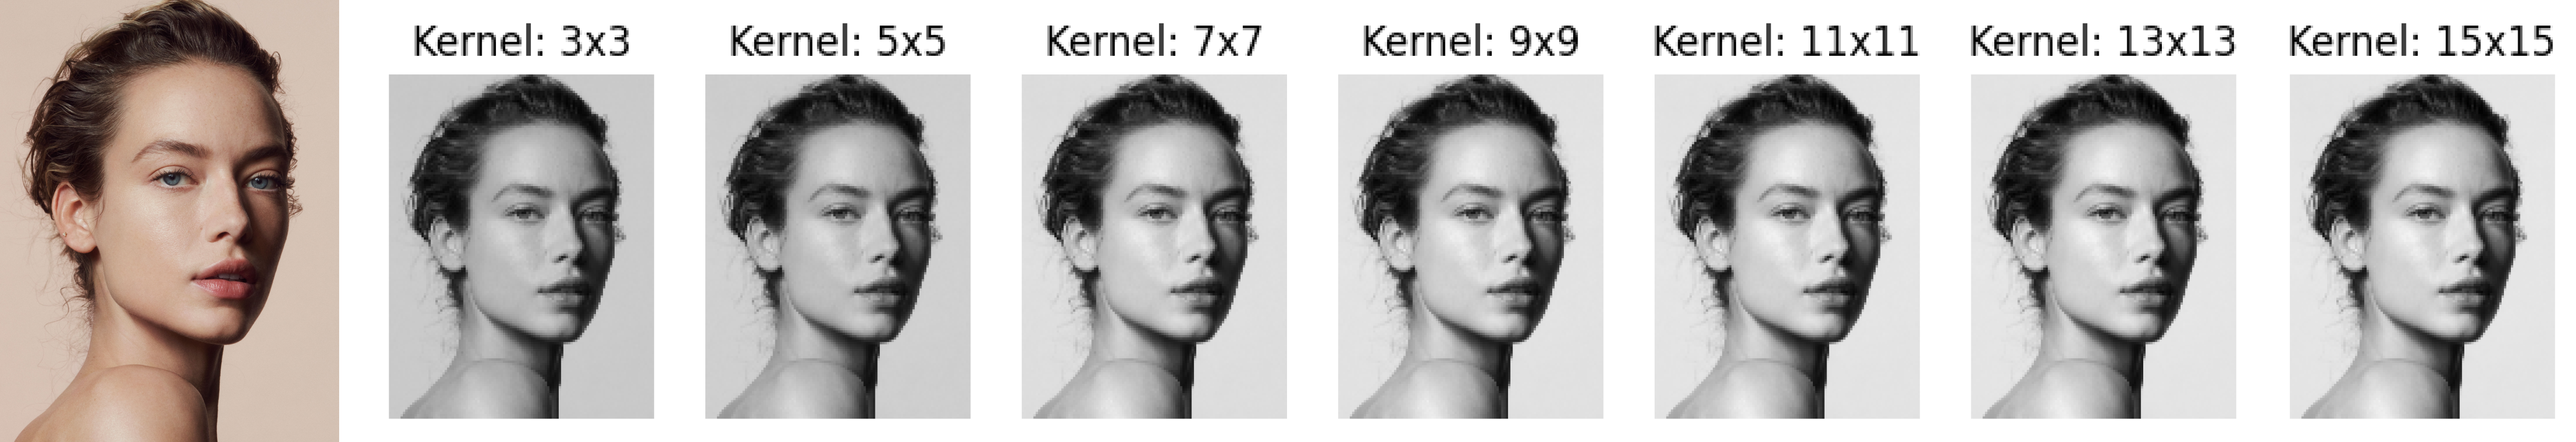
\includegraphics[width=0.4\textwidth]{images/Exp-4-Results-1.png} % Placeholder for results image
    \caption{Box Filtering}
    \label{fig:exp-4-results}
\end{figure}
    \item Defocus blur created a natural out-of-focus effect, suitable for simulating depth of field.
    \begin{figure}[h!]
    \centering
    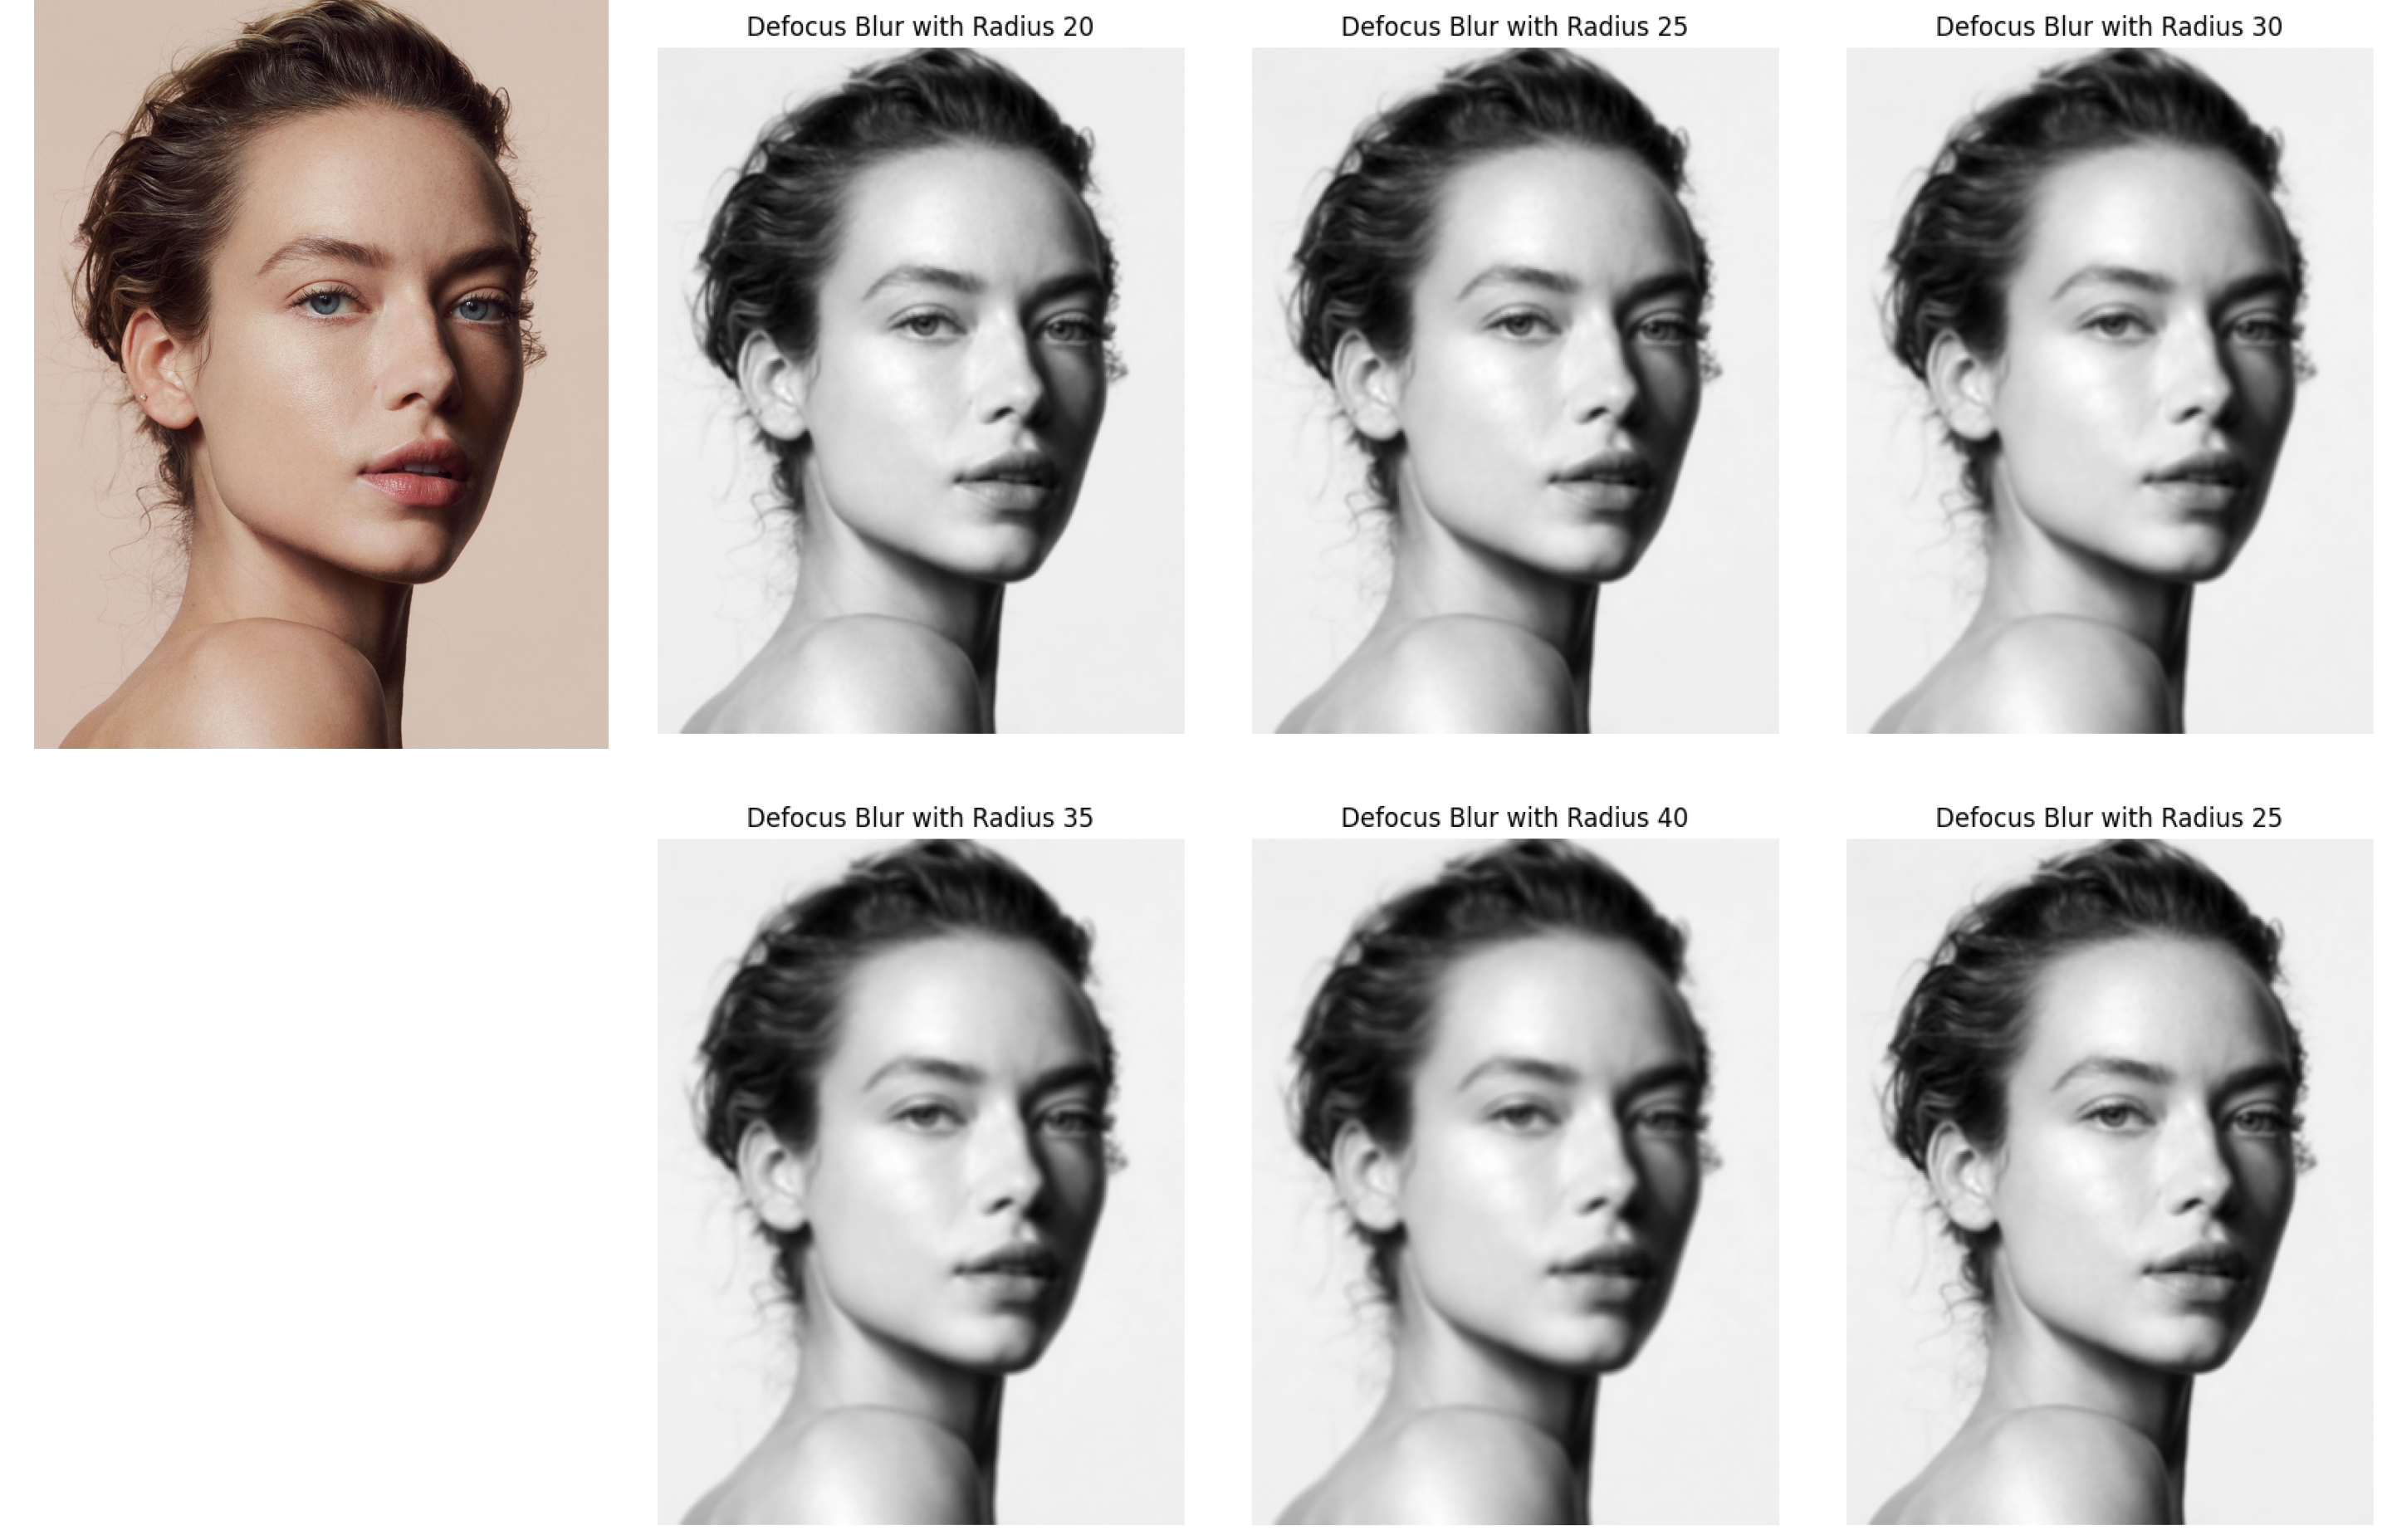
\includegraphics[width=0.4\textwidth]{images/Exp-4-Results-2.png} % Placeholder for results image
    \caption{Defocus Blurring}
    \label{fig:exp-4-results}
\end{figure}
    \item Motion blur simulated linear motion, demonstrating how camera movement affects image clarity.
    \begin{figure}[h!]
    \centering
    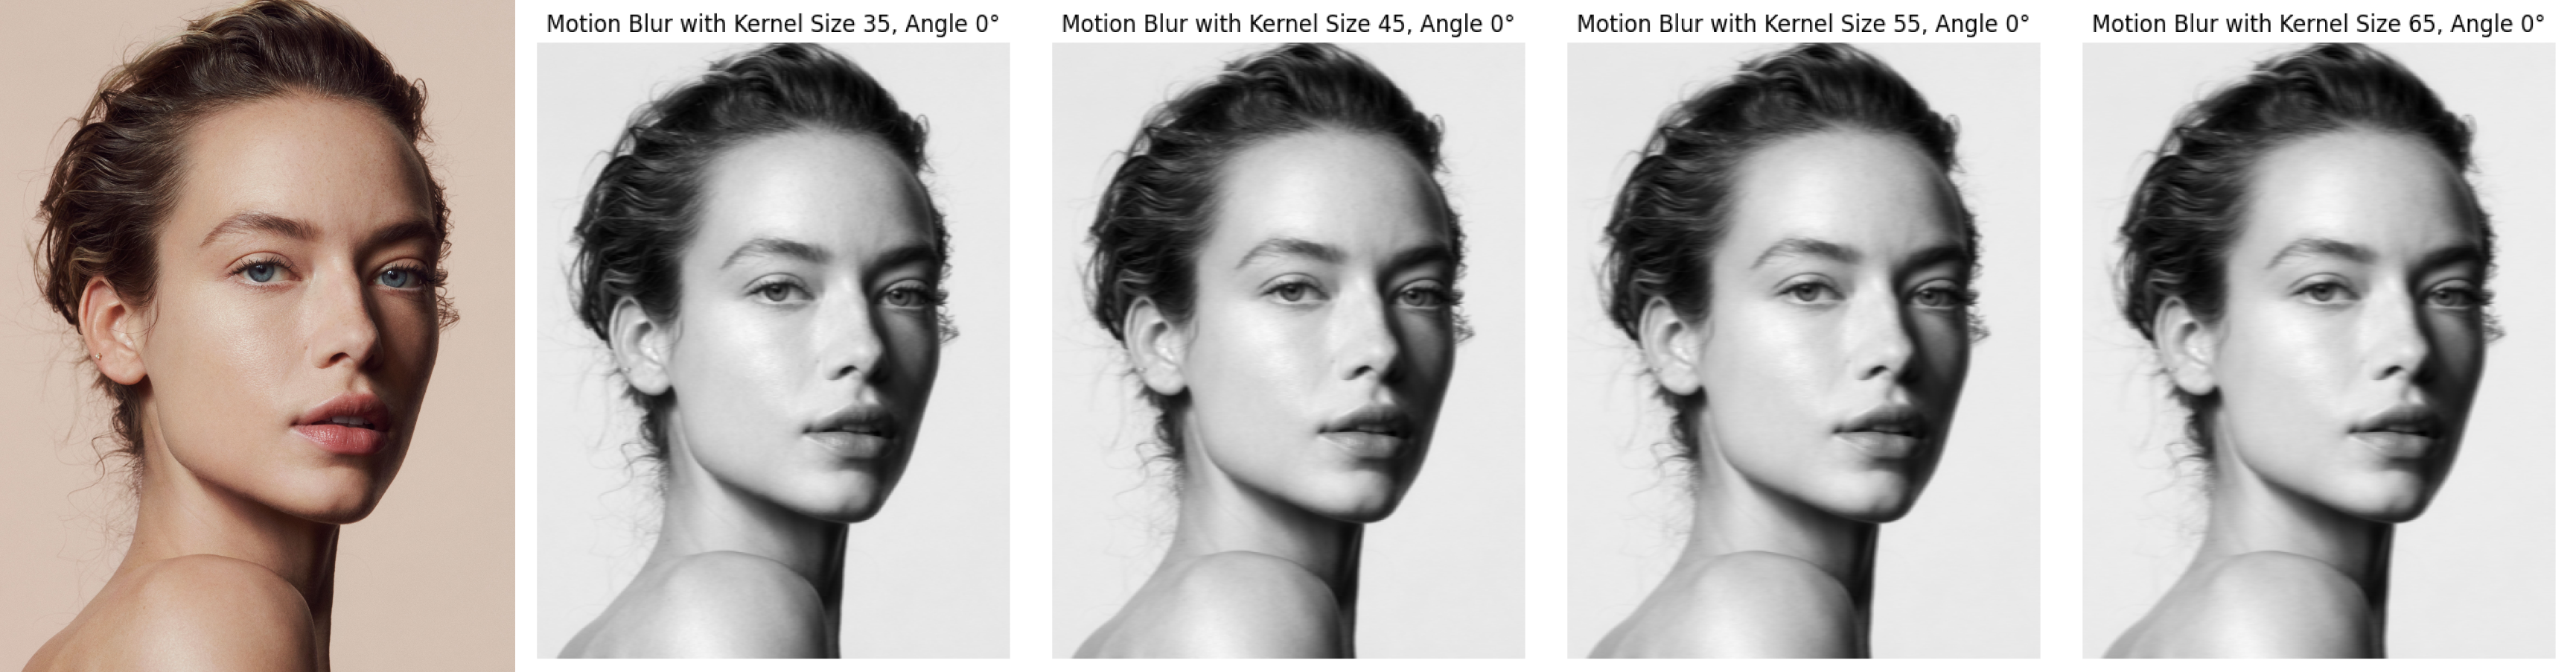
\includegraphics[width=0.4\textwidth]{images/Exp-4-Results-3.png} % Placeholder for results image
    \caption{Motion Blurring}
    \label{fig:exp-4-results}
\end{figure}
    \item Correlation and convolution produced distinct results, highlighting the impact of kernel flipping in convolution.
        \begin{figure}[h!]
    \centering
    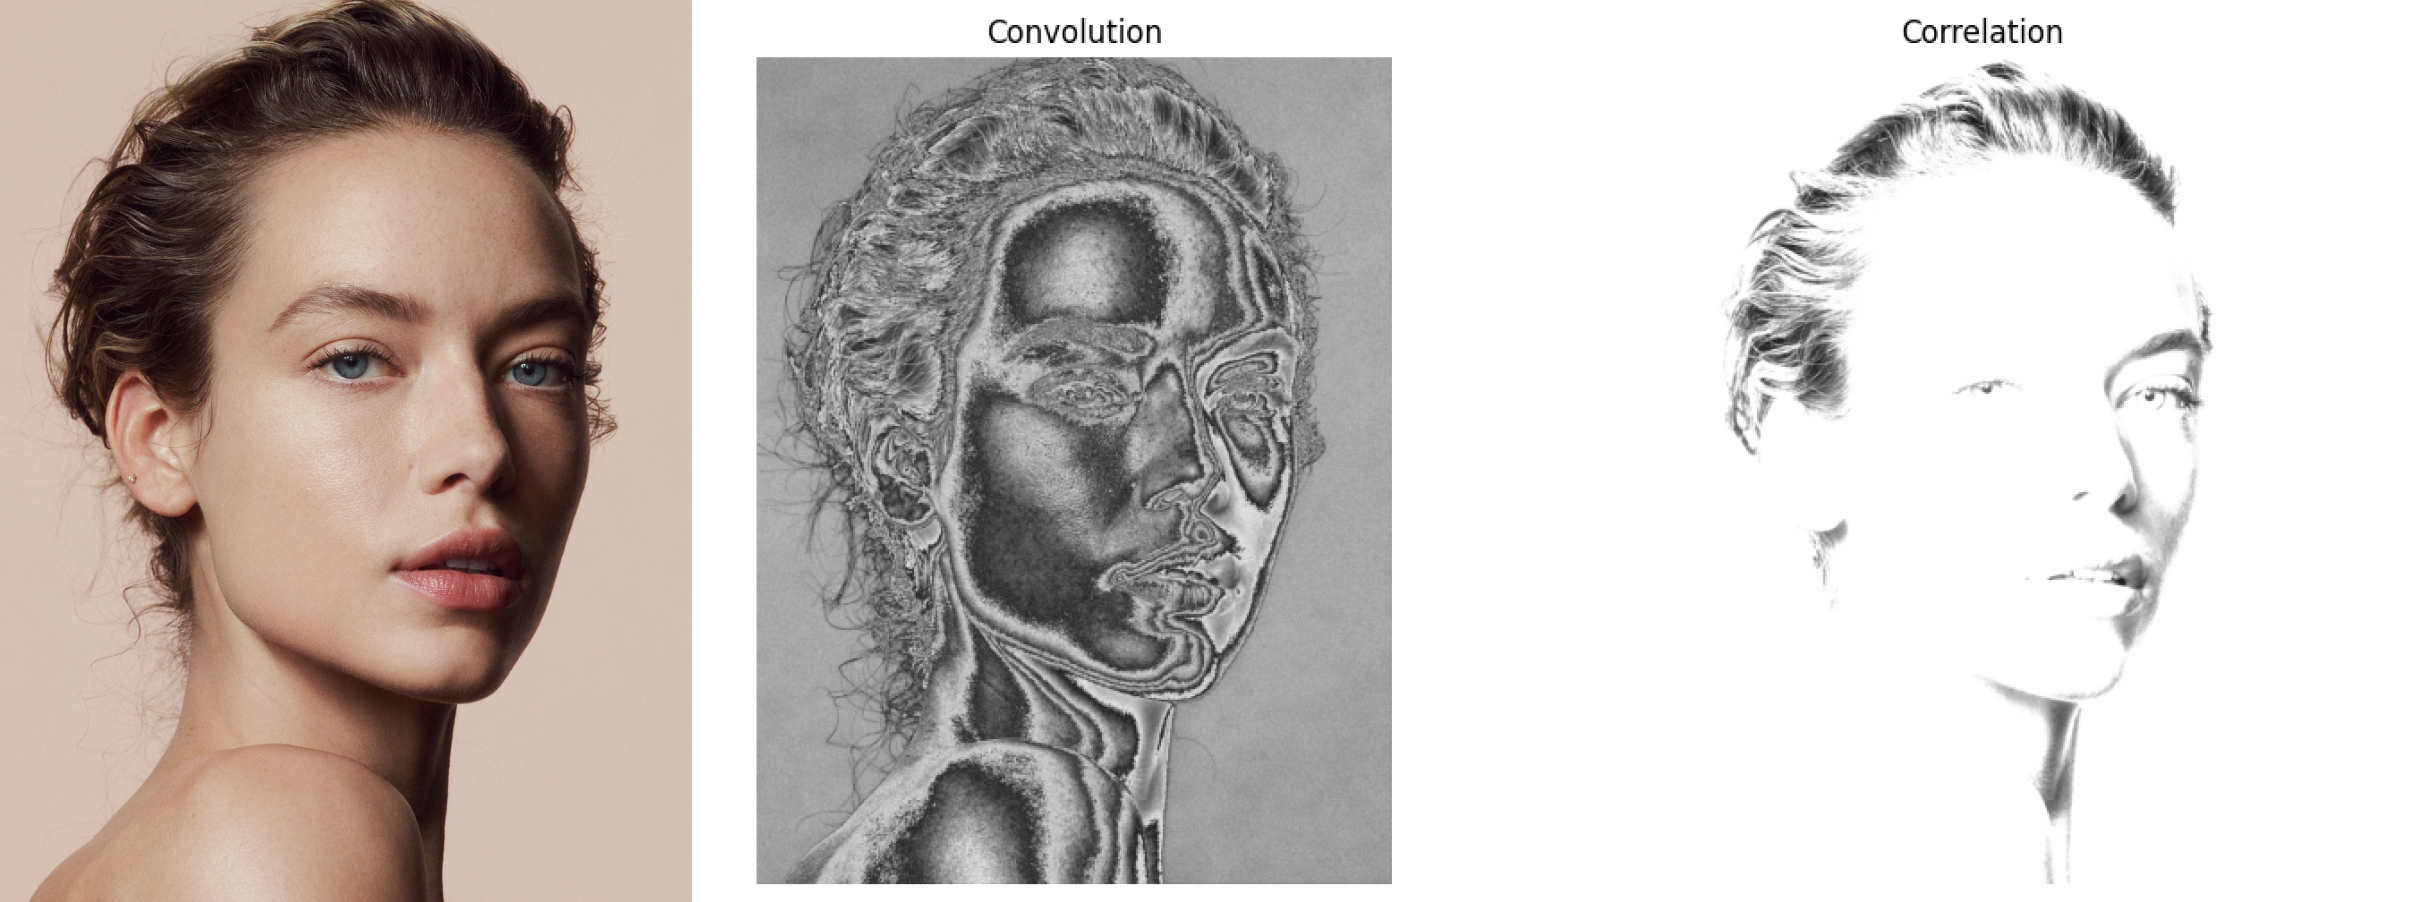
\includegraphics[width=0.4\textwidth]{images/Exp-4-Results-4.png} % Placeholder for results image
    \caption{Correlation vs Convolution}
    \label{fig:exp-4-results}
\end{figure}
    \item Separable filters significantly reduced computational overhead while producing similar results to non-separable filters.
    \begin{figure}[h!]
    \centering
    \includegraphics[width=0.4\textwidth]{images/Exp-4-Results-5.png} % Placeholder for results image
    \caption{Correlation vs Convolution}
    \label{fig:exp-4-results}
\end{figure}
    \item Gaussian Distribution with different sigma values
        \begin{figure}[h!]
    \centering
    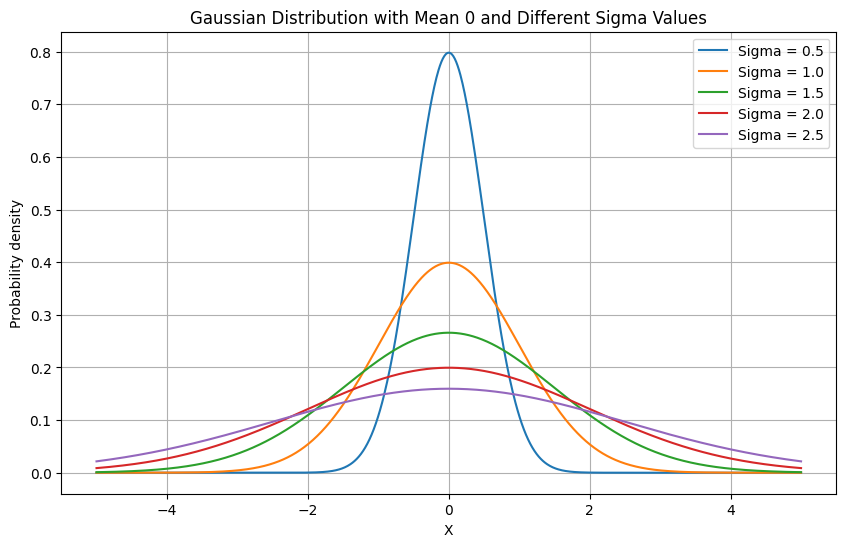
\includegraphics[width=0.4\textwidth]{images/Exp-4-Results-6.png} % Placeholder for results image
    \caption{Gaussian Distribution}
    \label{fig:exp-4-results}
\end{figure}
\end{itemize}

\section{Conclusion}
This experiment explored various image filtering and blurring techniques, providing insights into their applications and computational trade-offs. Future work could involve applying these techniques to real-world images and comparing their effectiveness.

\chapter{Experiment 5 - Gaussian Kernels} % Enable numbering for chapter

\section{Abstract}
This report documents the implementation of Gaussian filtering techniques on images. The experiment involves applying Gaussian blur, generating points from a standard normal distribution, and adding Gaussian noise to images. The goal is to understand the impact of Gaussian kernels in image processing.

\section{Introduction}
Gaussian filters are widely used in image processing to reduce noise and smooth images. This experiment applies Gaussian blurring and noise to images and visualizes the standard normal distribution.

\section{Methodology}
\subsection{Tools and Libraries}
\begin{itemize}
    \item \textbf{OpenCV}: For image processing operations.
    \item \textbf{NumPy}: For generating Gaussian noise.
    \item \textbf{Matplotlib}: For visualization.
\end{itemize}

\subsection{Implementation Steps}
\begin{enumerate}
    \item Read the input image in grayscale.
    \item Apply Gaussian blur using a $5\times5$ kernel.
    \item Generate data from a standard normal distribution and visualize the histogram.
    \item Add Gaussian noise to the image and display the results.
\end{enumerate}

\section{Implementation}
The implementation was carried out using Python with OpenCV and NumPy. The following code snippets demonstrate the processing steps:

\subsection{Applying Gaussian Blur}
\begin{lstlisting}[language=Python, caption=Gaussian Blur, label=code:gaussian-blur]
import cv2
import numpy as np
import matplotlib.pyplot as plt

image = cv2.imread('/content/fox_sample.jpeg', cv2.IMREAD_GRAYSCALE)
blurred_image = cv2.GaussianBlur(image, (5, 5), 0)
cv2.imwrite('blurred_image.jpg', blurred_image)
plt.imshow(blurred_image, cmap='gray')
plt.title('Gaussian Blurred Image')
plt.show()
\end{lstlisting}

\subsection{Generating Points from Standard Normal Distribution}
\begin{lstlisting}[language=Python, caption=Histogram of Standard Normal Distribution, label=code:normal-distribution]
data = np.random.randn(10000)

plt.hist(data, bins=50, density=True, alpha=0.6, color='g')
plt.title("Histogram of Standard Normal Distribution")
plt.xlabel("Value")
plt.ylabel("Frequency")
plt.show()
\end{lstlisting}

\subsection{Adding Gaussian Noise to an Image}
\begin{lstlisting}[language=Python, caption=Adding Gaussian Noise, label=code:gaussian-noise]
mean = 0
sigma = 25
gaussian_noise = np.random.normal(mean, sigma, image.shape)
noisy_image = np.clip(image + gaussian_noise, 0, 255).astype(np.uint8)

cv2.imwrite('noisy_image.jpg', noisy_image)
plt.imshow(noisy_image, cmap='gray')
plt.title('Image with Gaussian Noise')
plt.show()
\end{lstlisting}

\section{Results and Discussion}
The results from the experiment are summarized as follows:
\begin{itemize}
    \item The Gaussian blur effectively smoothens the image while preserving edges.
    \begin{figure}[h!]
    \centering
    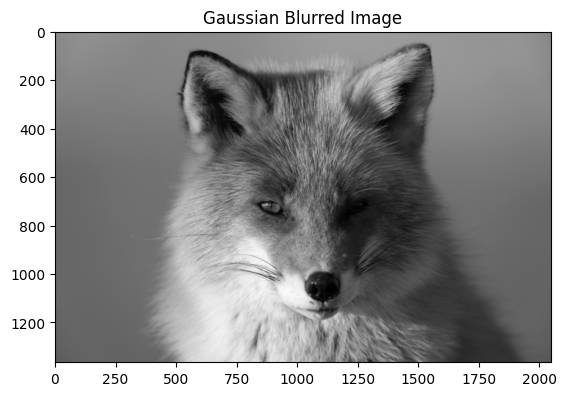
\includegraphics[width=0.4\textwidth]{images/Exp-5-Results-1.png} % Adjusted image size
    \caption{Gaussian Blurred Image.}
    \label{fig:blurred}
\end{figure}
    \item The histogram of the standard normal distribution follows the expected bell-shaped curve.
    \begin{figure}[h!]
    \centering
    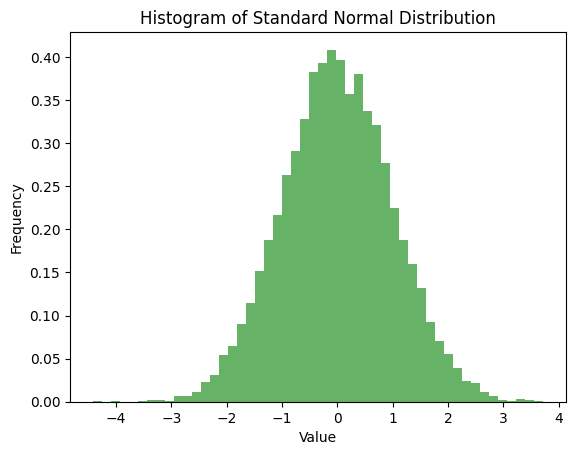
\includegraphics[width=0.4\textwidth]{images/Exp-5-Results-2.png} % Adjusted image size
    \caption{Image with Gaussian Noise.}
    \label{fig:noisy}
\end{figure}
    \item Adding Gaussian noise alters the image by introducing controlled randomness.
\end{itemize}
\begin{figure}[h!]
    \centering
    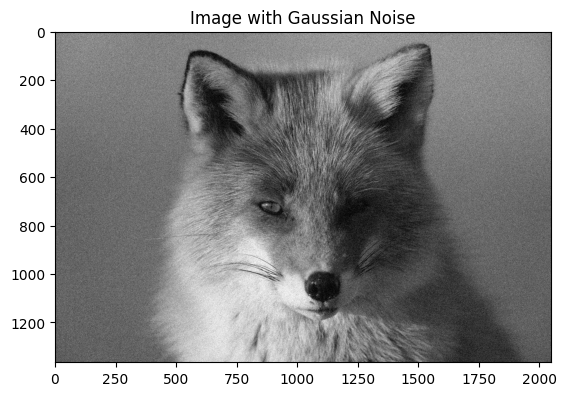
\includegraphics[width=0.4\textwidth]{images/Exp-5-Results-3.png} % Adjusted image size
    \caption{Image with Gaussian Noise.}
    \label{fig:noisy}
\end{figure}

\section{Conclusion}
This experiment successfully demonstrated the application of Gaussian kernels in image processing. Gaussian filtering effectively smoothens images, while Gaussian noise simulates real-world distortions. Future enhancements could include adaptive filtering techniques to preserve important image features while removing noise.

\chapter{Experiment 6 - Histogram Equalization}

\section{Introduction}
Histogram equalization is a technique used to enhance the contrast of an image by redistributing pixel intensity values. This experiment involves obtaining the histogram of an image, performing histogram equalization, comparing the original and equalized images, and modifying histograms through contrast stretching and histogram specification.

\section{Methodology}

\subsection{Histogram Computation}
To analyze the intensity distribution, the histogram of the grayscale image is computed using pixel intensity values.

\subsection{Histogram Equalization}
Histogram equalization is performed to spread intensity values across the full range, enhancing contrast.

\subsection{Comparison of Original and Equalized Images}
The original and equalized images are visually compared along with their histograms.

\subsection{Histogram Modification}
Contrast stretching and histogram specification are applied to modify the image’s histogram for better contrast adjustment.

\section{Implementation}
The experiment was implemented using Python and OpenCV. The following steps were performed:

\begin{itemize}
    \item Load a grayscale image.
    \item Compute and plot the histogram of the original image.
    \item Apply histogram equalization and plot the equalized histogram.
    \item Compare the original and equalized images with their histograms.
    \item Perform contrast stretching to enhance contrast.
    \item Implement histogram specification using a reference histogram.
\end{itemize}

\section{Code Implementation}

\lstset{language=Python, basicstyle=\ttfamily\small, keywordstyle=\color{blue}, commentstyle=\color{green}, stringstyle=\color{red}, frame=single, breaklines=true}

\begin{lstlisting}
import cv2
import numpy as np
import matplotlib.pyplot as plt

def plot_histogram(image, title, subplot_pos):
    plt.subplot(1, 2, subplot_pos)
    plt.hist(image.ravel(), bins=256, range=[0, 256], color='black')
    plt.title(title)
    plt.xlabel("Pixel Value")
    plt.ylabel("Frequency")

image = cv2.imread('sample.jpeg', cv2.IMREAD_GRAYSCALE)
plt.figure(figsize=(12, 5))
plot_histogram(image, "Histogram", 1)
plt.show()

# Histogram Equalization
image = cv2.imread('sample.jpeg', cv2.IMREAD_GRAYSCALE)
equalized_image = cv2.equalizeHist(image)
plt.figure(figsize=(12, 5))
plot_histogram(equalized_image, "Equalized Histogram", 2)
plt.show()

# Contrast Stretching
def contrast_stretching(image):
    min_val = np.min(image)
    max_val = np.max(image)
    stretched = ((image - min_val) / (max_val - min_val) * 255).astype(np.uint8)
    return stretched

stretched_image = contrast_stretching(image)

plt.figure(figsize=(15, 5))
plt.subplot(1, 4, 1)
plt.imshow(image, cmap='gray')
plt.title("Original Image")
plt.axis("off")

plt.subplot(1, 4, 2)
plt.imshow(stretched_image, cmap='gray')
plt.title("Contrast Stretched")
plt.axis("off")
plt.show()
\end{lstlisting}

\section{Results}

\begin{figure}[h!]
    \centering
    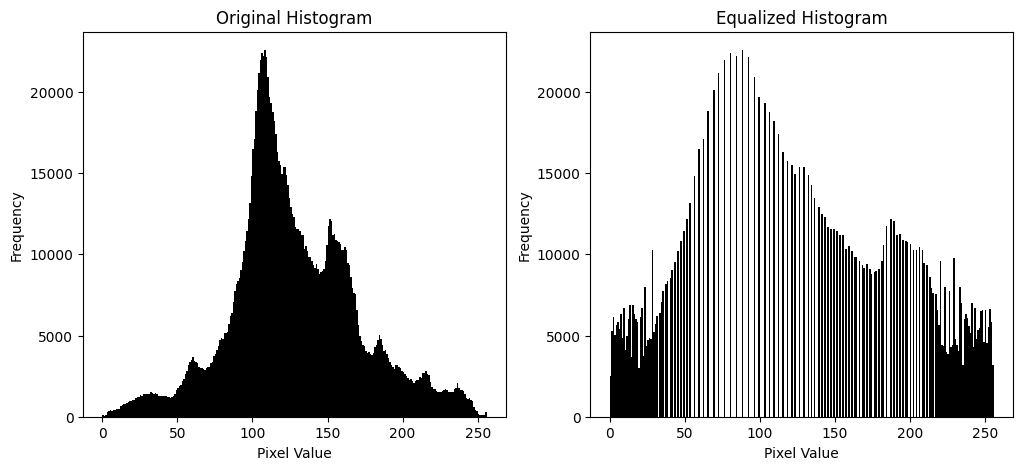
\includegraphics[width=\textwidth]{images/Exp-6-Results-4.png}
    \caption{Comparison between original and equalized histogram}
    \label{fig:noisy}
\end{figure}

\begin{figure}[h]
    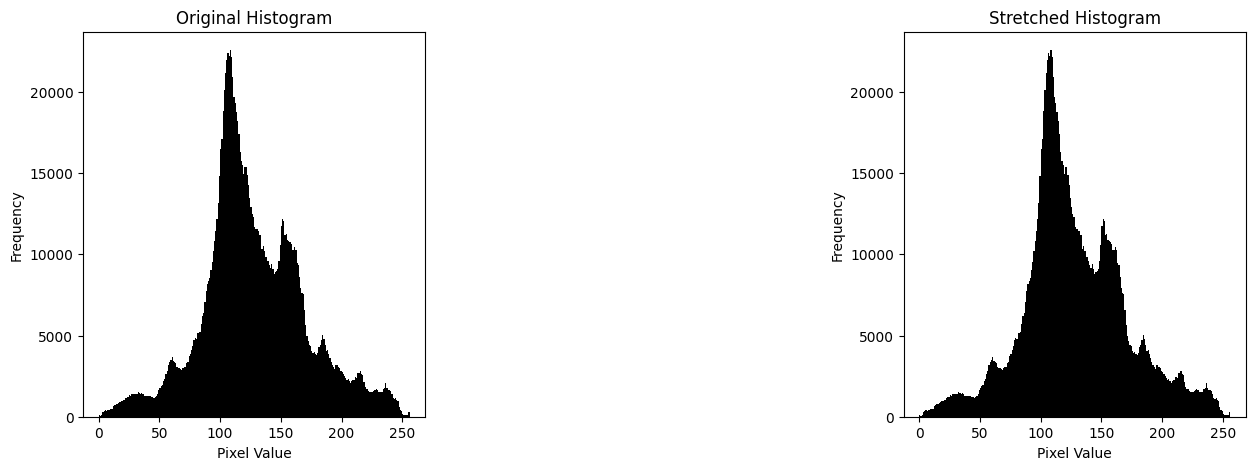
\includegraphics[width=\textwidth]{images/Exp-6-Results-3.png}
    \caption{Comparison of Image Transformations}
    \label{fig:noisy}
\end{figure}

\section{Conclusion}
Histogram equalization enhances image contrast by redistributing pixel intensities. Contrast stretching and histogram specification provide additional means for modifying image contrast based on specific requirements. The results demonstrate significant improvement in image visibility and details.

\chapter{Experiment 7 - Frequency Domain Filters}

\section{Introduction}
Frequency domain filtering is a fundamental technique in image processing where an image is transformed into the frequency domain using the Fourier Transform. The frequency components are modified using different filters before transforming back to the spatial domain. This experiment explores box filters, Gaussian filters, and low-pass filters in the frequency domain.

\section{Methodology}

\subsection{Fourier Transform}
The Fourier Transform converts an image into its frequency components, allowing filtering operations to be applied selectively.

\subsection{Filter Types}
\begin{itemize}
    \item \textbf{Box Filter}: A simple frequency domain filter that retains all frequencies within a specified cutoff.
    \item \textbf{Gaussian Filter}: Uses a Gaussian function to smoothly attenuate frequencies beyond the cutoff.
    \item \textbf{Low-Pass Filter}: Retains only low-frequency components, removing high-frequency details.
\end{itemize}

\section{Implementation}
The experiment was implemented using Python with OpenCV and NumPy. The following steps were performed:

\begin{itemize}
    \item Load a grayscale image.
    \item Apply Fourier Transform to obtain frequency domain representation.
    \item Create and apply filters (Box, Gaussian, and Low-Pass).
    \item Perform inverse Fourier Transform to obtain filtered images.
    \item Display results and compare effects of different filters.
\end{itemize}

\section{Code Implementation}

\lstset{language=Python, basicstyle=\ttfamily\small, keywordstyle=\color{blue}, commentstyle=\color{green}, stringstyle=\color{red}, frame=single, breaklines=true}

\begin{lstlisting}
import cv2
import numpy as np
import matplotlib.pyplot as plt

def apply_filter(image, filter_type, cutoff):
    if len(image.shape) == 3:
        image = cv2.cvtColor(image, cv2.COLOR_BGR2GRAY)

    rows, cols = image.shape
    crow, ccol = rows // 2, cols // 2

    dft = np.fft.fft2(image)
    dft_shift = np.fft.fftshift(dft)
    magnitude_spectrum = np.log(1 + np.abs(dft_shift))

    mask = np.zeros((rows, cols), np.float32)
    
    for u in range(rows):
        for v in range(cols):
            D = np.sqrt((u - crow) ** 2 + (v - ccol) ** 2)
            if filter_type == 'box':
                mask[u, v] = 1 if D <= cutoff else 0
            elif filter_type == 'gaussian':
                mask[u, v] = np.exp(-(D**2) / (2 * (cutoff**2)))
            elif filter_type == 'lowpass':
                mask[u, v] = 1 if D <= cutoff else 0
    
    filtered_dft = dft_shift * mask
    dft_ishift = np.fft.ifftshift(filtered_dft)
    img_back = np.fft.ifft2(dft_ishift)
    img_back = np.abs(img_back)
    
    return magnitude_spectrum, mask, np.log(1 + np.abs(filtered_dft)), img_back

image = cv2.imread('sample.jpg', cv2.IMREAD_GRAYSCALE)
filters = ['box', 'gaussian', 'lowpass']
cutoff = 50

fig, axs = plt.subplots(len(filters), 4, figsize=(16, 12))

for i, filter_type in enumerate(filters):
    F_uv, H_uv, G_uv, result = apply_filter(image, filter_type, cutoff)

    axs[i, 0].imshow(F_uv, cmap='gray')
    axs[i, 0].set_title(f'F(u,v) - {filter_type}')
    axs[i, 0].axis('off')

    axs[i, 1].imshow(H_uv, cmap='gray')
    axs[i, 1].set_title(f'H(u,v) - {filter_type}')
    axs[i, 1].axis('off')

    axs[i, 2].imshow(G_uv, cmap='gray')
    axs[i, 2].set_title(f'G(u,v) - {filter_type}')
    axs[i, 2].axis('off')

    axs[i, 3].imshow(result, cmap='gray')
    axs[i, 3].set_title(f'Inverse Transform - {filter_type}')
    axs[i, 3].axis('off')

plt.tight_layout()
plt.show()
\end{lstlisting}

\section{Results}

\begin{figure}[h]
    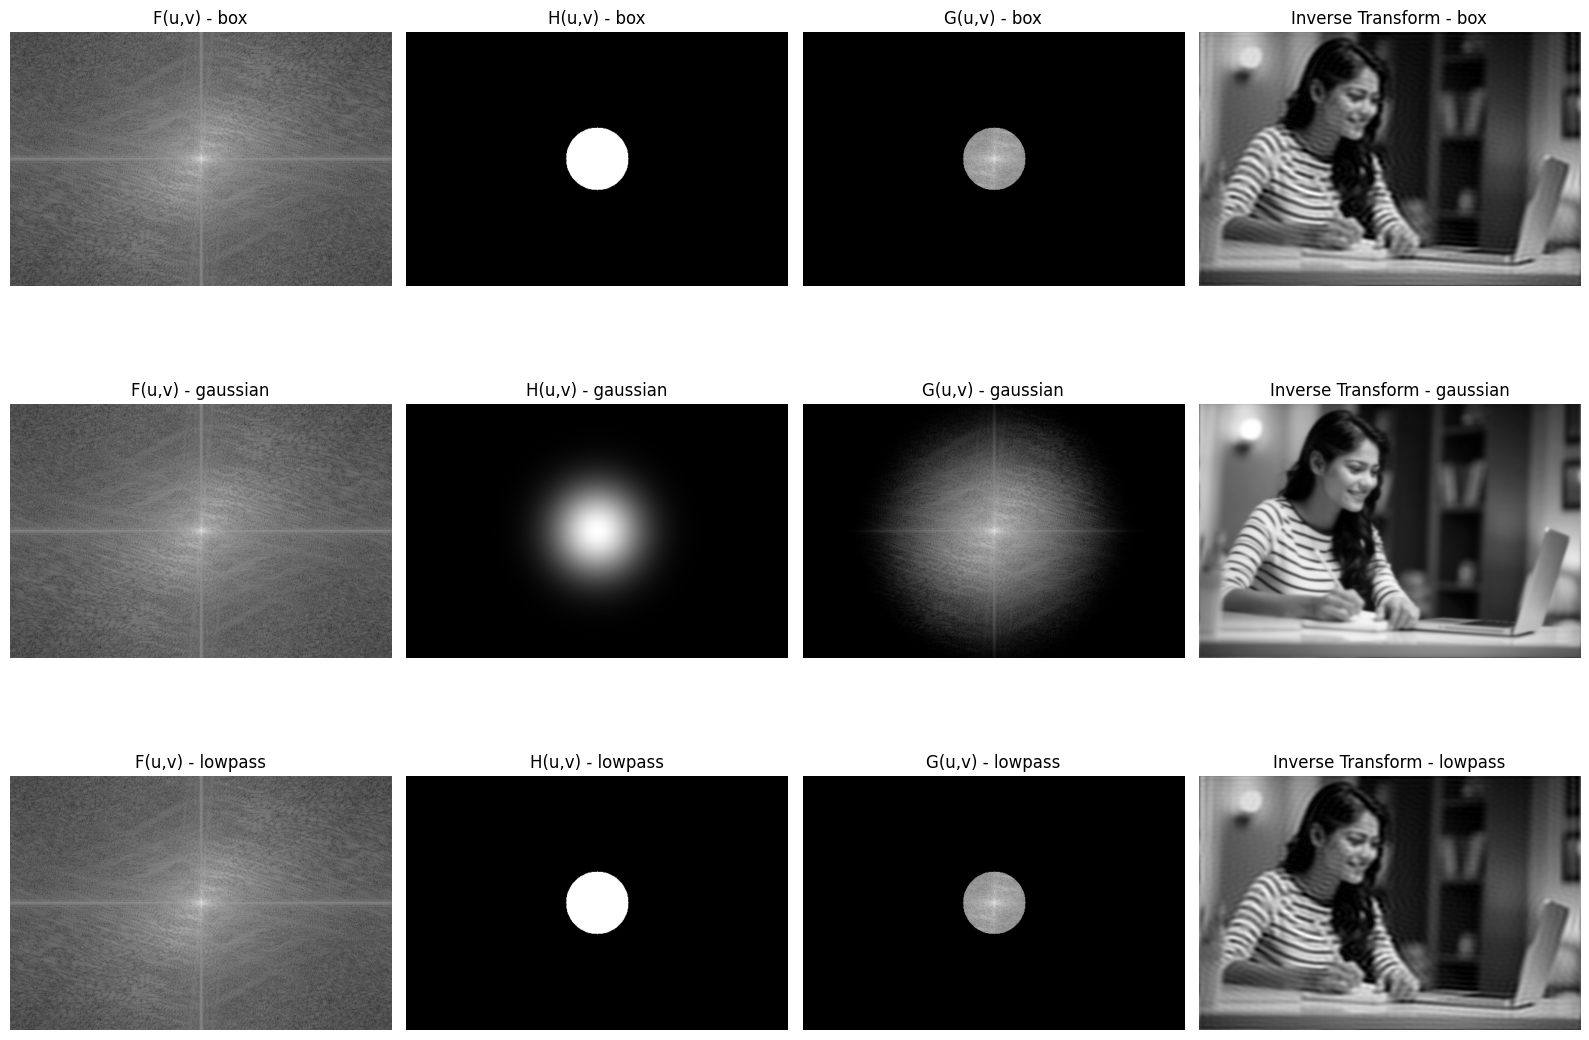
\includegraphics[width=\textwidth]{images/Exp-7-Results-1.png}
    \caption{Comparison of Image Transformations}
    \label{fig:noisy}
\end{figure}

\section{Conclusion}
Frequency domain filtering allows selective modification of image frequency components. The experiment demonstrated how box, Gaussian, and low-pass filters affect image frequency content. Gaussian filtering provided smoother transitions, whereas box filtering retained sharp cutoffs. These techniques are essential for applications in image enhancement and noise reduction.

\end{document}
